\documentclass[]{book}
\usepackage{lmodern}
\usepackage{amssymb,amsmath}
\usepackage{ifxetex,ifluatex}
\usepackage{fixltx2e} % provides \textsubscript
\ifnum 0\ifxetex 1\fi\ifluatex 1\fi=0 % if pdftex
  \usepackage[T1]{fontenc}
  \usepackage[utf8]{inputenc}
\else % if luatex or xelatex
  \ifxetex
    \usepackage{mathspec}
  \else
    \usepackage{fontspec}
  \fi
  \defaultfontfeatures{Ligatures=TeX,Scale=MatchLowercase}
\fi
% use upquote if available, for straight quotes in verbatim environments
\IfFileExists{upquote.sty}{\usepackage{upquote}}{}
% use microtype if available
\IfFileExists{microtype.sty}{%
\usepackage{microtype}
\UseMicrotypeSet[protrusion]{basicmath} % disable protrusion for tt fonts
}{}
\usepackage[left=3cm,right=3cm,top=3cm,bottom=3cm]{geometry}
\usepackage{hyperref}
\hypersetup{unicode=true,
            pdftitle={Biostatistics in Public Health},
            pdfauthor={Ralph Trane},
            pdfborder={0 0 0},
            breaklinks=true}
\urlstyle{same}  % don't use monospace font for urls
\usepackage{natbib}
\bibliographystyle{apalike}
\usepackage{longtable,booktabs}
\usepackage{graphicx,grffile}
\makeatletter
\def\maxwidth{\ifdim\Gin@nat@width>\linewidth\linewidth\else\Gin@nat@width\fi}
\def\maxheight{\ifdim\Gin@nat@height>\textheight\textheight\else\Gin@nat@height\fi}
\makeatother
% Scale images if necessary, so that they will not overflow the page
% margins by default, and it is still possible to overwrite the defaults
% using explicit options in \includegraphics[width, height, ...]{}
\setkeys{Gin}{width=\maxwidth,height=\maxheight,keepaspectratio}
\IfFileExists{parskip.sty}{%
\usepackage{parskip}
}{% else
\setlength{\parindent}{0pt}
\setlength{\parskip}{6pt plus 2pt minus 1pt}
}
\setlength{\emergencystretch}{3em}  % prevent overfull lines
\providecommand{\tightlist}{%
  \setlength{\itemsep}{0pt}\setlength{\parskip}{0pt}}
\setcounter{secnumdepth}{5}
% Redefines (sub)paragraphs to behave more like sections
\ifx\paragraph\undefined\else
\let\oldparagraph\paragraph
\renewcommand{\paragraph}[1]{\oldparagraph{#1}\mbox{}}
\fi
\ifx\subparagraph\undefined\else
\let\oldsubparagraph\subparagraph
\renewcommand{\subparagraph}[1]{\oldsubparagraph{#1}\mbox{}}
\fi

%%% Use protect on footnotes to avoid problems with footnotes in titles
\let\rmarkdownfootnote\footnote%
\def\footnote{\protect\rmarkdownfootnote}

%%% Change title format to be more compact
\usepackage{titling}

% Create subtitle command for use in maketitle
\providecommand{\subtitle}[1]{
  \posttitle{
    \begin{center}\large#1\end{center}
    }
}

\setlength{\droptitle}{-2em}

  \title{Biostatistics in Public Health}
    \pretitle{\vspace{\droptitle}\centering\huge}
  \posttitle{\par}
    \author{Ralph Trane}
    \preauthor{\centering\large\emph}
  \postauthor{\par}
      \predate{\centering\large\emph}
  \postdate{\par}
    \date{Fall 2019(last compiled: 2019-09-27)}


\begin{document}
\maketitle

{
\setcounter{tocdepth}{1}
\tableofcontents
}
\hypertarget{introduction-to-notes}{%
\chapter{Introduction to Notes}\label{introduction-to-notes}}

\newcommand{\Var}{\text{Var}}
\newcommand{\var}{\text{var}}
\newcommand{\SD}{\text{SD}}

Welcome to Public Health 783. This is where you'll find my notes for the biostatistics part of this class for Fall 2019.

These notes are meant to be a supplement to lectures and \citet{ls}. If you have any doubts as to what parts of the book I think are more important, this is a good place to look. There's a good chance that if it is not included here, I do not care too much about it. That being said, things included here might not be elaborated to a satisfying extent, and therefore I do \emph{NOT} recommend that you rely solely on these notes, but rather use them in conjunction with the book, and, just as importantly, lectures.

I want to emphasize that these notes are not exhaustive, but are meant to complement lectures. We simply won't have time to cover everything in the amount of detail I would like. Therefore, I will use these notes to write down some thoughts on certain topics that I think you might as well read outside the classroom. At times I will ask you to read sections before showing up to lectures. Other times, I won't even make the material available to you until after lectures. There's good reason for that. Some things are easier to explain when you have already seen them before. Other concepts can be scary on paper, and are best introduced by another human being. In either case, it is extremely important that you show up to lectures.

Finally, note that this collection is a living thing. It will change throughout the semester as we move along. Sometimes I might go back and clarify sections, if it seems to be necessary. At the beginning of the class you'll only find the first part, but as we make our way through, I will publish more notes on the topics to be covered later.

\hypertarget{bounty-program}{%
\section*{Bounty Program}\label{bounty-program}}
\addcontentsline{toc}{section}{Bounty Program}

As already mentioned, this is a living document. Furthermore, it is very much so the first version. Therefore, there will inevitably be mistakes. Hopefully, most of them will be minor, but I would be surprised if there isn't a few major ones here and there. Therefore, I really hope that you will all help me out and let me know whenever you find mistakes, no matter how small they might seem.

Now, I know that noone wants to do that -- who has the time to send an email just to let some fool know they can't spell ``stastitics''. But it's important to me to gradually improve these notes, and often being made aware of small mistakes opens up ones eyes to bigger ones. So to incentivize you to report mistakes, I have decided to start a bounty program: if you as a group gather more than 20 points (see below on how to collect points), there will be a reward at the end of the semester! If you find a mistake, simply shoot me an \href{mailto:rtrane@wisc.edu}{email}, let me know where the mistake is, and what type you think it is.

\begin{longtable}[]{@{}ll@{}}
\toprule
Type of Mistake & Points\tabularnewline
\midrule
\endhead
Spelling/grammatical error & 1\tabularnewline
Math error & 2\tabularnewline
Conceptual nonsense in either text or math & 3\tabularnewline
\bottomrule
\end{longtable}

\hypertarget{intro}{%
\chapter{Introduction to Biostatistics}\label{intro}}

\hypertarget{what-is-biostatistics}{%
\section{What is Biostatistics?}\label{what-is-biostatistics}}

Biostatistics is ``simply'' statistics applied to a specific set of problems, namely problems related to biological questions. Hence, the question ``what is biostatistics?'' is quickly replaced by ``what is statistics?''

From Wikipedia\footnote{\ldots{} because where else do you go when you're not sure where to start?}: ``Statistics is the discipline that concerns the collection, organization, displaying, analysis, interpretation, and presentation of data.'' That is quite the range, but all it is saying is that statistics is the science of making sense of data.

It is very hard to pinpoint exactly what statistics is, but it is rather easy to dismiss at least one very common misunderstanding: statistics is \emph{NOT} an exact science. There is (almost) never just one answer to a question. Rather, statistics is a decision science in the sense that at every step of the way, from study design to data collection to data presentation to data analysis and interpretation, you have to make decisions. And inevitably, your conclusions depend on every single one of those decisions.

\hypertarget{biostatistics-in-publhlth-783}{%
\section{Biostatistics in PUBLHLTH 783}\label{biostatistics-in-publhlth-783}}

In this class, we'll be considering what might seem like a very simple setup with simple questions, and a general approach to answering said questions. The truth is basically all statistical methods, no matter how complicated they might seem, follow (to some extend) this exact pattern. In this class, we will work our way through this pattern, and talk about how the simplest of methods work. The hope is that when we're done, you take these simple methods with you, and whenever you encounter more complicated methods, you can draw parallels back to what you have seen here, which hopefully will help you make at least some sense of even the most complicated methods.

The story begins\ldots{}

Any statistical analysis begins with a research question. This question always relates to a certain \emph{feature} or \emph{characteristic} of a certain \emph{population}, or of multiple populations. The population is the group of entities one wants to learn more about. It could be that one is interested in the life expectancy (feature) of U.S. adults (population), risk of diabetes (feature) among people with a certain genetic profile (population), the resistance to a disease (feature) among ants in Governor Dodge State Park (population), strength (feature) of pipes produced by a certain manufacturer (population), etc.

Now, the first fundamental idea of the approach we'll pursue in this class is this: there is a single true answer to the question asked. The only one way to obtain the truth is to observe the entire population. If we could measure the disease status (diabetes/no diabetes) of every single individual with the genetic profile of interest, we could evaluate the true risk. The catch is, maybe obviously to someone, that this is simply not feasible. Often we do not even know exactly how big the population of interest is, which means it is impossible to survey every single subject in the population. And even if we knew exactly how many people were part of the population, how to get a hold of them, and how to convince them to participate in our study, it is very unlikely we would have the resources (read: \$\$\$) to reach out and include every single one of them.

This leads us to the picture we will return to over and over again in this class: there is some population of interest. We want to say something about a certain feature of the population. This will usually be a mean of a measurement, the risk ratio or odds ratio of two groups, or something similar. Unfortunately, there is no way we can actually measure the feature for every single subject in the population -- if we could, we would simply calculate the mean, and be done with it! Instead, we take a \emph{sample} from the population. The hope is that we obtain this sample in such a way that the sample is representative of the entire population, and therefore we can use the information obtained from the sample to say something about the population.

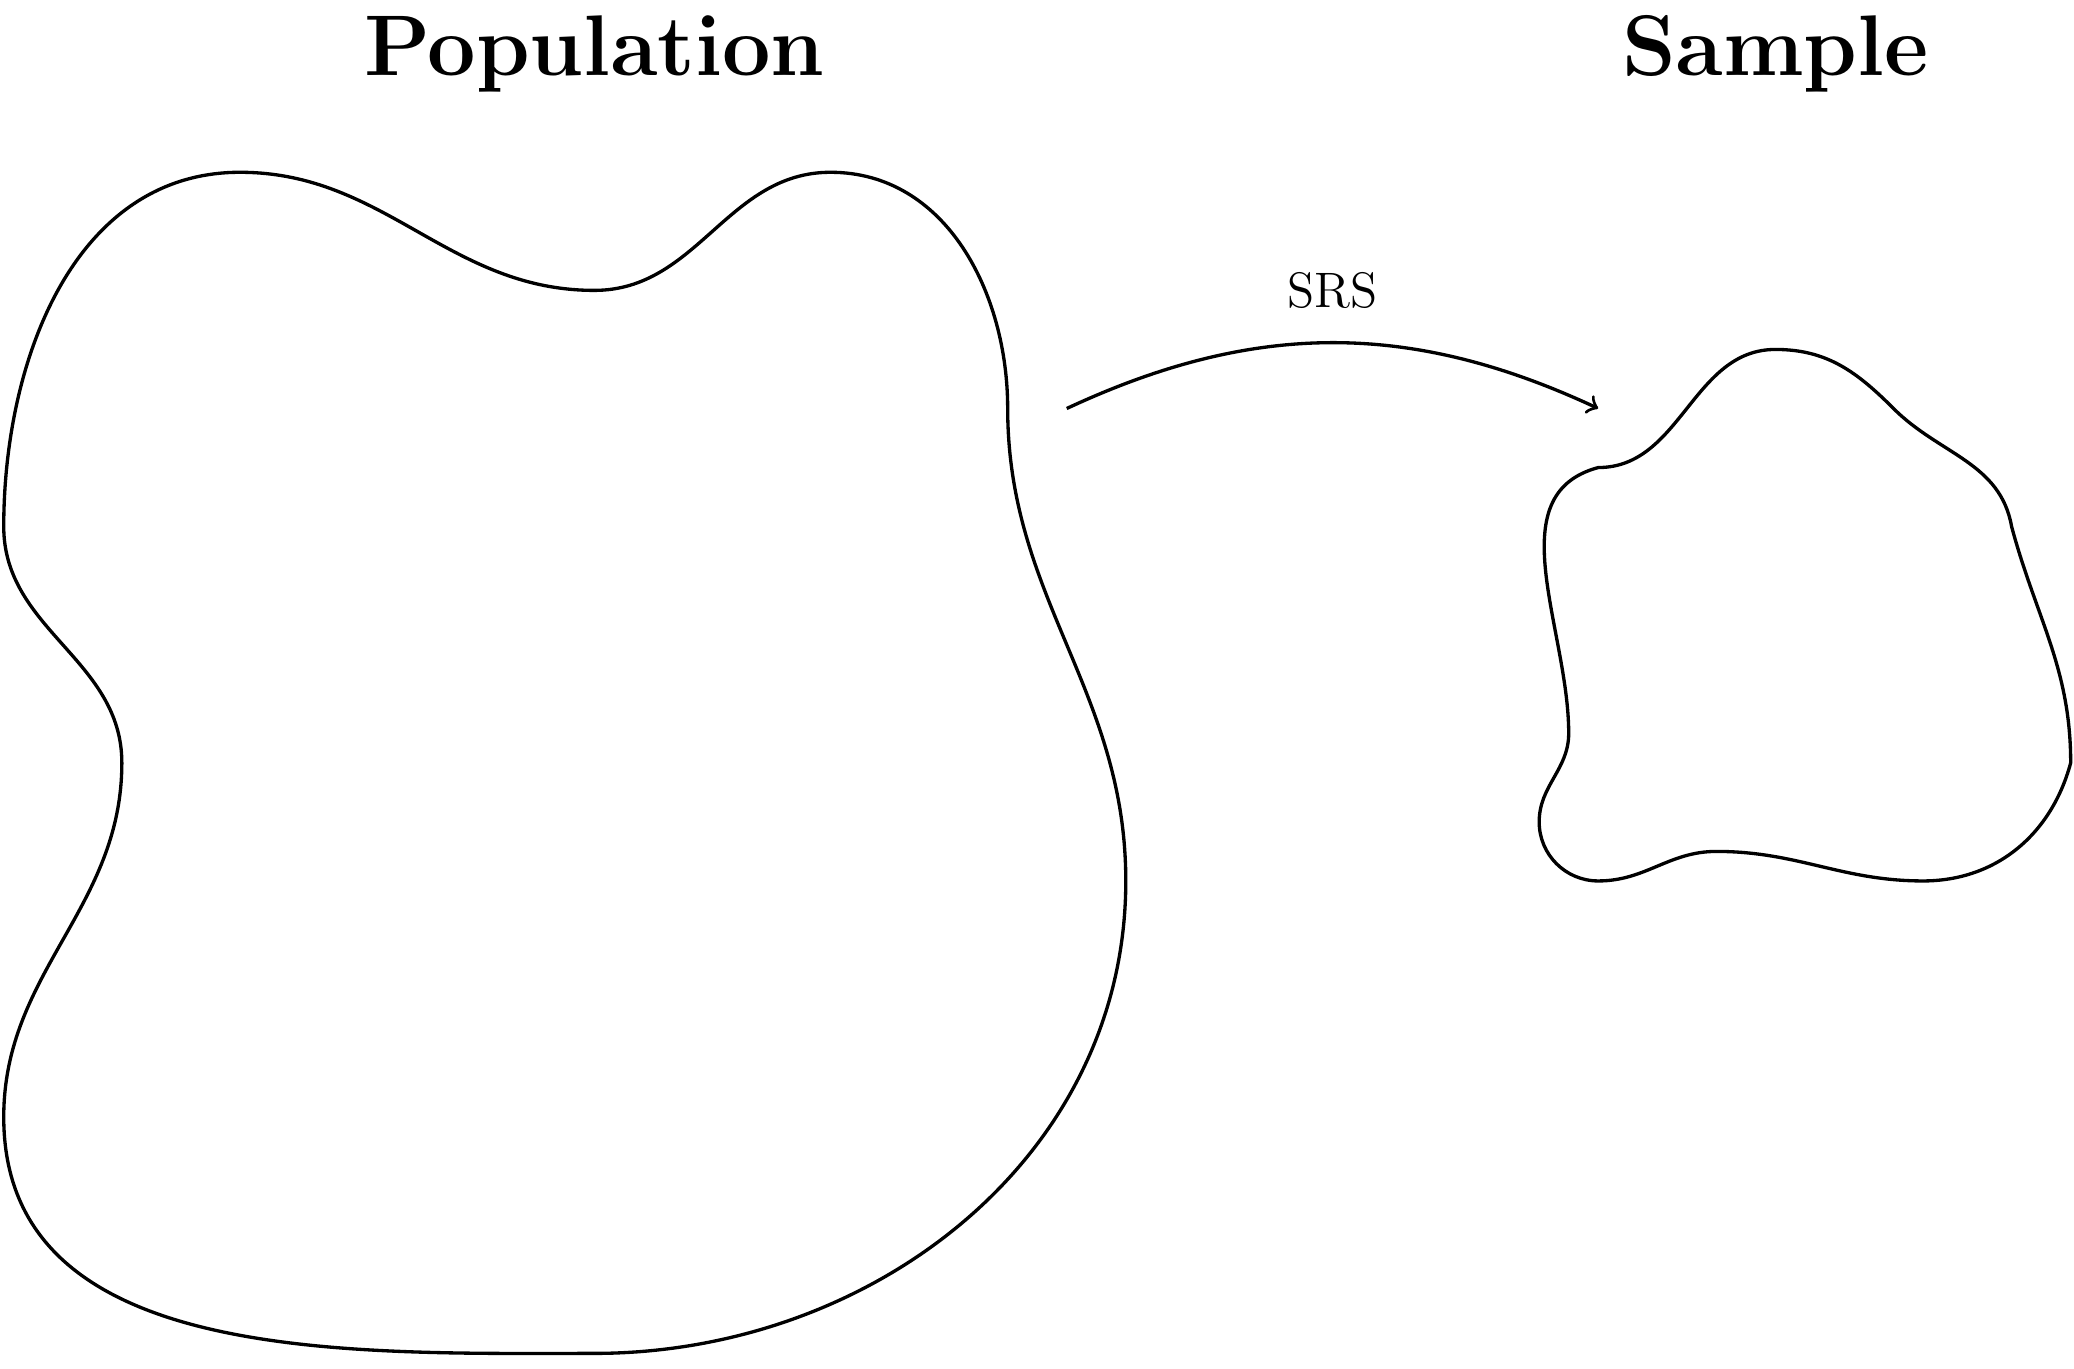
\includegraphics{783_biostats_files/figure-latex/unnamed-chunk-3-1.pdf}

When we talk about chances of observing something when sampling from the population, we talk about \emph{probabilities}. What is the probability a sample of 23 people has more than 5 diabetics? What is the probability a randomly chosen individual from Minneapolis will develop cancer?

When we try to use a sample to say something about the general population from which the sample was created, we do \emph{inference}.

The plot thickens\ldots{}

We now have an idea of what it is we want to do: take a sample, obtain some information about the thing of interest, then use that information to say something about the general population. Pretty simple. The problem is, how do we actually put the pieces together in a way that allows us to generalize to the population? Example: we are interested in estimating the prevalence of cardiovascular disease in the general population of U.S. adults. We have a hunch that the true prevalence is 11\%. We take a sample of 3799 female U.S. adults of which 379 have a history of CVD. So, the prevalence is estimated to be \(\frac{379}{3799} \approx 10 \%\)\footnote{This data was obtained from the Framingham Offspring Study, see table 3-1, page 24 of \citet{ls}}. The prevalence in our sample is clearly different from our hypothesis, so clearly our hypothesis is wrong\ldots. right?

If only it was that simple. The problem here is that our prevalence estimate depends on the specific sample we got. If we were to repeat this experiment, we would ask a different group of people about their history of CVD, which would lead to a different estimate of the prevalence. There's simply no way (or it is at least very, very unlikely) we'll ever get a sample of people for which the prevalence matches our hypothesis exactly. So the question is not simply if our sample has the same prevalence as hypothesized, but rather is it ``close enough'' for us to believe our hypothesis.

Close enough? Did I read that right?

Yup. The majority of statistical methods, and definitely everything we'll be talking about in this class, are trying to decide if what we observe in our sample is ``close enough'' to our hypothesize about the population. The idea is that if what we observe is very far from our hypothesis, then it is unlikely that the hypothesis is true.

There are generally two ways of framing the question:

\begin{enumerate}
\def\labelenumi{\arabic{enumi}.}
\tightlist
\item
  Is what we observe (think prevalence in sample) ``close enough'' to the hypothesis (that the prevalence in the population is 11\%)?
\item
  What range of hypotheses (values for the prevalence) would we accept given what we observed?
\end{enumerate}

The first approach is refered to as testing a \emph{statistical hypothesis}, or \emph{null hypothesis significance testing} (NHST), while the second is refered to as constructing a \emph{confidence interval}. These two are closely related, as we will see later, but the information contained in the results differ drastically. While testing a hypothesis only provides you with a result concerning \textbf{one value}, the confidence interval gives you a wide range of values that you to some extent believe could be the true value. Why would anyone then ever report the result of a statistical hypothesis test without a confidence interval, you ask? That is a very, very, very good question to which I do not have an answer\ldots{}

This has all been very abstract (and I think I got carried away in that last paragraph). We'll see examples of this over and over again throughout the semester, so hopefully it'll be easier to comprehend as we go along.

\hypertarget{part-data-types-and-descriptive-statistics}{%
\part{Data Types and Descriptive Statistics}\label{part-data-types-and-descriptive-statistics}}

\hypertarget{before-we-get-started}{%
\chapter{Before we get started\ldots{}}\label{before-we-get-started}}

This section is very minimal. I decided to go that route because 1) this is the ``easiest'' part of the material in the sense that there isn't a lot of things to really understand and think about, and 2) it is objectively speaking very, very, very boring\ldots{} So, when you find my notes insufficient, take a look at Chapter 4 in \citep{ls}.

\textbf{Learning Objectives}

\begin{enumerate}
\def\labelenumi{\arabic{enumi}.}
\item
  Understand why descriptive statistics is important, and useful
\item
  Know the difference between discrete and continuous variables/data
\item
  Have some ideas of which summaries and figures are appropriate for different types of data
\end{enumerate}

\hypertarget{why-descriptive-statistics}{%
\chapter{Why Descriptive Statistics?}\label{why-descriptive-statistics}}

\emph{Descriptive Statistics}, as the name implies, are about describing something. In general, we can only describe what we have at hand, so descriptive statistics only deal with the population in the very, very, very rare case when we have measured the entire population. It is way more common that descriptive statistics are about the sample at hand.

Often when conducting an experiment, what we are actually interested in is using the sample we obtain to say something about the general population. If we, for example, enroll 200 patients in a study to find out if a new drug works, we're not \emph{really} interested in whether or not it works for those 200 patients specifically, but more so if it works for any individual from the population in general. With that in mind, the whole concept of descriptive statistics might not seem very (1) exciting, (2) useful, or (3) necessary. While (1) is highly subjective, (2) very much so depends on the specific situation, there is little question that it is in fact necessary.

Recall our general setup for any statistical analysis: we have some question about some feature of a population. To answer this question, we go get a sample of the population. If this is a good sample, the characteristics of this sample mimic those of the general population. If this is the case, then the hope is that we can draw conclusions about the sample, and generalize them to the general population. Conversely, if that is \emph{not} the case, then no matter how convincing the evidence we find in the sample is for or against our hypotheses, it tells us nothing about the general population.

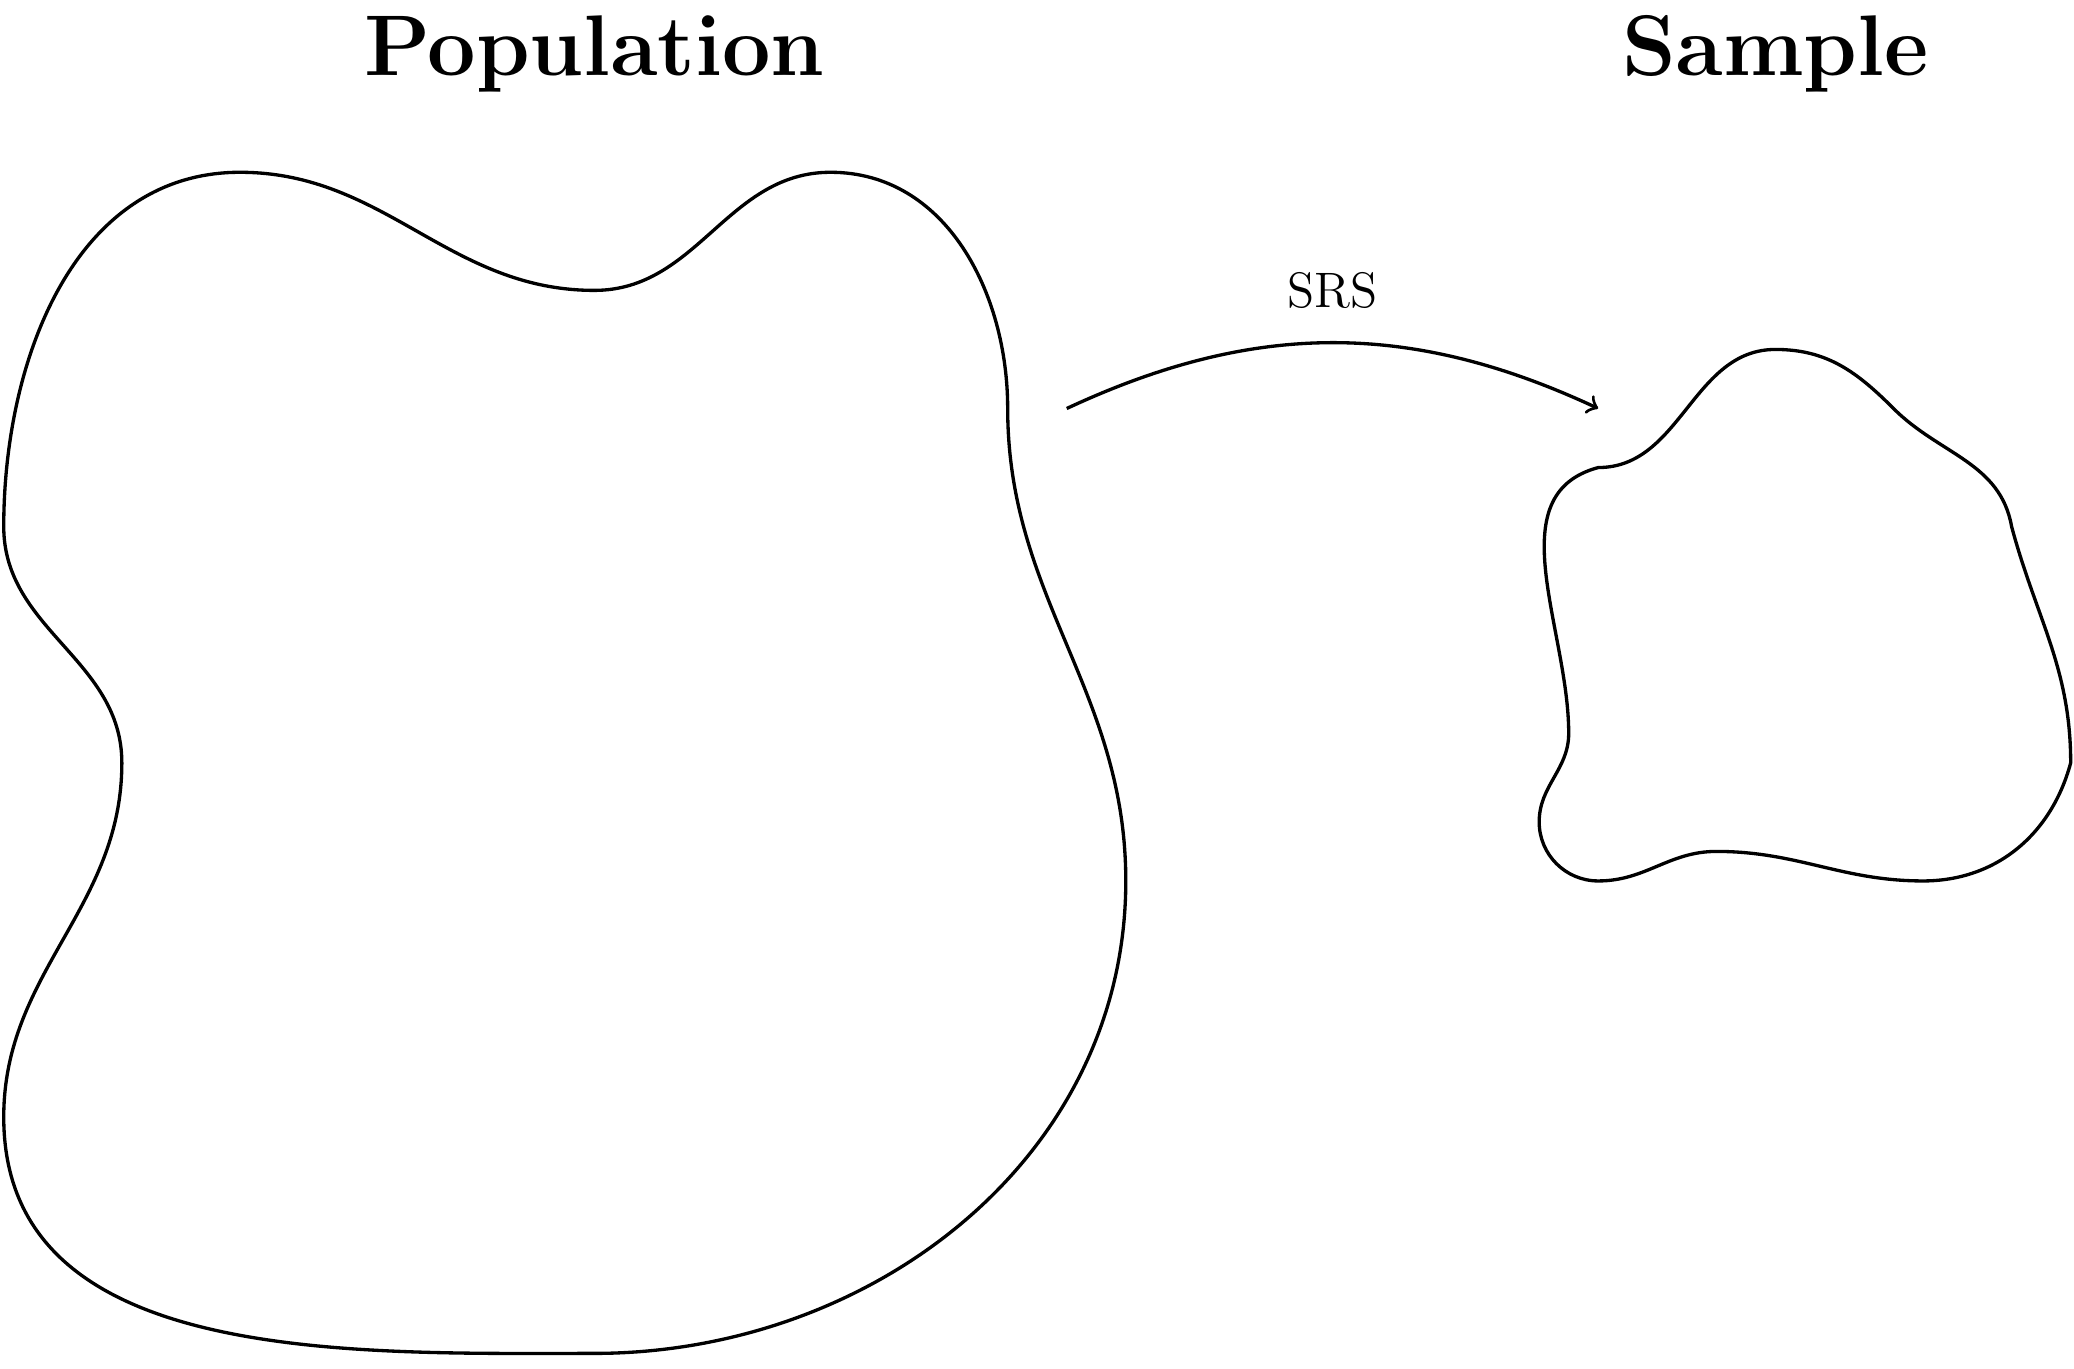
\includegraphics{783_biostats_files/figure-latex/general-population-1.pdf}

So how do we make sure the sample is representative of the population? The first step is to make sure our sampling scheme is good. Ideally, we sample completely at random, meaning that every single individual in the population has the same chance of ending up in the sample. As you might be able to guess, this is rarely the case, but if the sampling is done right it is either approximately true, or the sampling is done in a way that any biases introduced can be accounted for in the analysis.\footnote{\textbf{Full disclaimer}: sampling is hard. As in really, really, really hard. Very smart people spend a lot of time on making sure different sampling schemes work. It is well beyond the scope of this course, and me, how the details of this work out.} Most commonly, sampling is done in such a way that the ``equal chance'' assumption isn't too crazy. But how do we know if this is actually the case?

The truth is, we don't really. What we can do, though, is describe the sample we obtain. That way we can make sure we don't generalize any results to an inappropriate population. Historically, this mistake has been made over and over again in medical research when excluding women and ethnic minorities from studies.\footnote{See \citet{liu_womens_2016} for a more thorough discussion of the exclusion of women in particular.} For this particular reason, producing descriptive statistics is often the first step in any data analysis.

The rest of this section will go through different types of data, and show how we, in each case, can describe (or summarize, if you will) the specific type of data.

In general, when we talk about data we often refer to \emph{variables}. Variables are simply (and very vaguely) \emph{things we measure}. You will see examples which hopefully helps understand exactly what is meant by a variable.

\hypertarget{discrete}{%
\chapter{Discrete Data}\label{discrete}}

A variable is called a \emph{discrete} variable if the possible values of the variable are countable, that is if you can count them. Note that a discrete variable can technically have an infinite number of possible outcomes.

A discrete variable is of one of two subtypes: \emph{categorical} or \emph{ordinal}.

\hypertarget{categorical}{%
\section{Categorical data}\label{categorical}}

Categorical variables are discrete variables with no particular ordering of the categories.

\hypertarget{examples-categorical-data}{%
\subsection{Examples -- categorical data}\label{examples-categorical-data}}

The classical example of a categorical variable is sex. For each subject, the value of this variable is one of two possible values: male or female.

Other examples:

\begin{itemize}
\tightlist
\item
  color
\item
  race
\item
  blood type
\item
  country of origin
\item
  political orientation
\end{itemize}

\hypertarget{binarydichotomous-data}{%
\subsection{Binary/Dichotomous Data}\label{binarydichotomous-data}}

Often researchers will refer to certain variables as \emph{binary} or \emph{dichotomous}. This simply means \emph{categorical with two categories}.

\hypertarget{how-to-describe-categorical-data}{%
\section{How to describe categorical data}\label{how-to-describe-categorical-data}}

Categorical variables are often described using \emph{frequency counts} and \emph{relative frequencies}.

\emph{Frequency counts} (or simply \emph{frequencies}) are found by counting how many times each possible value is present in the data. \emph{Relative frequencies} are found by dividing the frequency by the total number of observations.

\hypertarget{examples}{%
\subsection{Examples}\label{examples}}

Below are the frequencies for some categorical variables in the SHOW data set. One thing that often comes from this preliminary step of a data analysis is the realization that there are some kinks in your data. For example, notice how there are missing values for most of these variables (denoted by NA -- ``Not Available'').

\begin{itemize}
\item
  \textbf{edu}:

  \begin{longtable}[]{@{}cc@{}}
  \toprule
  \begin{minipage}[b]{0.41\columnwidth}\centering
  Value\strut
  \end{minipage} & \begin{minipage}[b]{0.16\columnwidth}\centering
  Frequency\strut
  \end{minipage}\tabularnewline
  \midrule
  \endhead
  \begin{minipage}[t]{0.41\columnwidth}\centering
  {[}0{]} Never
  attended/kindergarten only\strut
  \end{minipage} & \begin{minipage}[t]{0.16\columnwidth}\centering
  2\strut
  \end{minipage}\tabularnewline
  \begin{minipage}[t]{0.41\columnwidth}\centering
  {[}3{]} 3rd grade\strut
  \end{minipage} & \begin{minipage}[t]{0.16\columnwidth}\centering
  2\strut
  \end{minipage}\tabularnewline
  \begin{minipage}[t]{0.41\columnwidth}\centering
  {[}4{]} 4th grade\strut
  \end{minipage} & \begin{minipage}[t]{0.16\columnwidth}\centering
  1\strut
  \end{minipage}\tabularnewline
  \begin{minipage}[t]{0.41\columnwidth}\centering
  {[}6{]} 6th grade\strut
  \end{minipage} & \begin{minipage}[t]{0.16\columnwidth}\centering
  4\strut
  \end{minipage}\tabularnewline
  \begin{minipage}[t]{0.41\columnwidth}\centering
  {[}7{]} 7th grade\strut
  \end{minipage} & \begin{minipage}[t]{0.16\columnwidth}\centering
  2\strut
  \end{minipage}\tabularnewline
  \begin{minipage}[t]{0.41\columnwidth}\centering
  {[}8{]} 8th grade\strut
  \end{minipage} & \begin{minipage}[t]{0.16\columnwidth}\centering
  20\strut
  \end{minipage}\tabularnewline
  \begin{minipage}[t]{0.41\columnwidth}\centering
  {[}9{]} 9th grade\strut
  \end{minipage} & \begin{minipage}[t]{0.16\columnwidth}\centering
  22\strut
  \end{minipage}\tabularnewline
  \begin{minipage}[t]{0.41\columnwidth}\centering
  {[}10{]} 10th grade\strut
  \end{minipage} & \begin{minipage}[t]{0.16\columnwidth}\centering
  49\strut
  \end{minipage}\tabularnewline
  \begin{minipage}[t]{0.41\columnwidth}\centering
  {[}11{]} 11th grade\strut
  \end{minipage} & \begin{minipage}[t]{0.16\columnwidth}\centering
  66\strut
  \end{minipage}\tabularnewline
  \begin{minipage}[t]{0.41\columnwidth}\centering
  {[}12{]} 12th grade, No diploma\strut
  \end{minipage} & \begin{minipage}[t]{0.16\columnwidth}\centering
  90\strut
  \end{minipage}\tabularnewline
  \begin{minipage}[t]{0.41\columnwidth}\centering
  {[}13{]} High school graduate\strut
  \end{minipage} & \begin{minipage}[t]{0.16\columnwidth}\centering
  624\strut
  \end{minipage}\tabularnewline
  \begin{minipage}[t]{0.41\columnwidth}\centering
  {[}14{]} GED or equivalent\strut
  \end{minipage} & \begin{minipage}[t]{0.16\columnwidth}\centering
  112\strut
  \end{minipage}\tabularnewline
  \begin{minipage}[t]{0.41\columnwidth}\centering
  {[}15{]} Some college, no degree\strut
  \end{minipage} & \begin{minipage}[t]{0.16\columnwidth}\centering
  680\strut
  \end{minipage}\tabularnewline
  \begin{minipage}[t]{0.41\columnwidth}\centering
  {[}16{]} Associate degree:
  occupational, technical, or
  vocational program\strut
  \end{minipage} & \begin{minipage}[t]{0.16\columnwidth}\centering
  437\strut
  \end{minipage}\tabularnewline
  \begin{minipage}[t]{0.41\columnwidth}\centering
  {[}17{]} Associate degree:
  academic program\strut
  \end{minipage} & \begin{minipage}[t]{0.16\columnwidth}\centering
  191\strut
  \end{minipage}\tabularnewline
  \begin{minipage}[t]{0.41\columnwidth}\centering
  {[}18{]} Bachelor's degree\strut
  \end{minipage} & \begin{minipage}[t]{0.16\columnwidth}\centering
  723\strut
  \end{minipage}\tabularnewline
  \begin{minipage}[t]{0.41\columnwidth}\centering
  {[}19{]} Master's degree\strut
  \end{minipage} & \begin{minipage}[t]{0.16\columnwidth}\centering
  263\strut
  \end{minipage}\tabularnewline
  \begin{minipage}[t]{0.41\columnwidth}\centering
  {[}20{]} Professional degree\strut
  \end{minipage} & \begin{minipage}[t]{0.16\columnwidth}\centering
  47\strut
  \end{minipage}\tabularnewline
  \begin{minipage}[t]{0.41\columnwidth}\centering
  {[}21{]} Doctoral degree\strut
  \end{minipage} & \begin{minipage}[t]{0.16\columnwidth}\centering
  40\strut
  \end{minipage}\tabularnewline
  \begin{minipage}[t]{0.41\columnwidth}\centering
  {[}.D{]} Don't know\strut
  \end{minipage} & \begin{minipage}[t]{0.16\columnwidth}\centering
  1\strut
  \end{minipage}\tabularnewline
  \begin{minipage}[t]{0.41\columnwidth}\centering
  NA\strut
  \end{minipage} & \begin{minipage}[t]{0.16\columnwidth}\centering
  5\strut
  \end{minipage}\tabularnewline
  \bottomrule
  \end{longtable}
\item
  \textbf{gender}:

  \begin{longtable}[]{@{}cc@{}}
  \toprule
  \begin{minipage}[b]{0.17\columnwidth}\centering
  Value\strut
  \end{minipage} & \begin{minipage}[b]{0.17\columnwidth}\centering
  Frequency\strut
  \end{minipage}\tabularnewline
  \midrule
  \endhead
  \begin{minipage}[t]{0.17\columnwidth}\centering
  {[}1{]} Male\strut
  \end{minipage} & \begin{minipage}[t]{0.17\columnwidth}\centering
  1479\strut
  \end{minipage}\tabularnewline
  \begin{minipage}[t]{0.17\columnwidth}\centering
  {[}2{]} Female\strut
  \end{minipage} & \begin{minipage}[t]{0.17\columnwidth}\centering
  1901\strut
  \end{minipage}\tabularnewline
  \begin{minipage}[t]{0.17\columnwidth}\centering
  NA\strut
  \end{minipage} & \begin{minipage}[t]{0.17\columnwidth}\centering
  1\strut
  \end{minipage}\tabularnewline
  \bottomrule
  \end{longtable}
\item
  \textbf{marital}:

  \begin{longtable}[]{@{}cc@{}}
  \toprule
  \begin{minipage}[b]{0.34\columnwidth}\centering
  Value\strut
  \end{minipage} & \begin{minipage}[b]{0.16\columnwidth}\centering
  Frequency\strut
  \end{minipage}\tabularnewline
  \midrule
  \endhead
  \begin{minipage}[t]{0.34\columnwidth}\centering
  {[}1{]} Married\strut
  \end{minipage} & \begin{minipage}[t]{0.16\columnwidth}\centering
  2075\strut
  \end{minipage}\tabularnewline
  \begin{minipage}[t]{0.34\columnwidth}\centering
  {[}2{]} Widowed\strut
  \end{minipage} & \begin{minipage}[t]{0.16\columnwidth}\centering
  113\strut
  \end{minipage}\tabularnewline
  \begin{minipage}[t]{0.34\columnwidth}\centering
  {[}3{]} Divorced\strut
  \end{minipage} & \begin{minipage}[t]{0.16\columnwidth}\centering
  416\strut
  \end{minipage}\tabularnewline
  \begin{minipage}[t]{0.34\columnwidth}\centering
  {[}4{]} Separated\strut
  \end{minipage} & \begin{minipage}[t]{0.16\columnwidth}\centering
  41\strut
  \end{minipage}\tabularnewline
  \begin{minipage}[t]{0.34\columnwidth}\centering
  {[}5{]} Never married\strut
  \end{minipage} & \begin{minipage}[t]{0.16\columnwidth}\centering
  603\strut
  \end{minipage}\tabularnewline
  \begin{minipage}[t]{0.34\columnwidth}\centering
  {[}6{]} Living with partner\strut
  \end{minipage} & \begin{minipage}[t]{0.16\columnwidth}\centering
  126\strut
  \end{minipage}\tabularnewline
  \begin{minipage}[t]{0.34\columnwidth}\centering
  {[}.D{]} Don't know\strut
  \end{minipage} & \begin{minipage}[t]{0.16\columnwidth}\centering
  2\strut
  \end{minipage}\tabularnewline
  \begin{minipage}[t]{0.34\columnwidth}\centering
  NA\strut
  \end{minipage} & \begin{minipage}[t]{0.16\columnwidth}\centering
  5\strut
  \end{minipage}\tabularnewline
  \bottomrule
  \end{longtable}
\item
  \textbf{race}:

  \begin{longtable}[]{@{}cc@{}}
  \toprule
  \begin{minipage}[b]{0.41\columnwidth}\centering
  Value\strut
  \end{minipage} & \begin{minipage}[b]{0.16\columnwidth}\centering
  Frequency\strut
  \end{minipage}\tabularnewline
  \midrule
  \endhead
  \begin{minipage}[t]{0.41\columnwidth}\centering
  {[}1{]} Non-hispanic white\strut
  \end{minipage} & \begin{minipage}[t]{0.16\columnwidth}\centering
  2870\strut
  \end{minipage}\tabularnewline
  \begin{minipage}[t]{0.41\columnwidth}\centering
  {[}2{]} Non-hispanic African
  American\strut
  \end{minipage} & \begin{minipage}[t]{0.16\columnwidth}\centering
  243\strut
  \end{minipage}\tabularnewline
  \begin{minipage}[t]{0.41\columnwidth}\centering
  {[}3{]} Hispanic\strut
  \end{minipage} & \begin{minipage}[t]{0.16\columnwidth}\centering
  108\strut
  \end{minipage}\tabularnewline
  \begin{minipage}[t]{0.41\columnwidth}\centering
  {[}4{]} Other race or ethinicity\strut
  \end{minipage} & \begin{minipage}[t]{0.16\columnwidth}\centering
  151\strut
  \end{minipage}\tabularnewline
  \begin{minipage}[t]{0.41\columnwidth}\centering
  NA\strut
  \end{minipage} & \begin{minipage}[t]{0.16\columnwidth}\centering
  9\strut
  \end{minipage}\tabularnewline
  \bottomrule
  \end{longtable}
\end{itemize}

We can add relative frequencies to this simply by dividing each frequency by the total number of observations. You can check a few of them yourself -- simply divide the frequency by the total number of observations (found on the last line of the table).

\begin{itemize}
\item
  \textbf{edu}:

  \begin{longtable}[]{@{}ccc@{}}
  \toprule
  \begin{minipage}[b]{0.39\columnwidth}\centering
  Value\strut
  \end{minipage} & \begin{minipage}[b]{0.15\columnwidth}\centering
  Frequency\strut
  \end{minipage} & \begin{minipage}[b]{0.27\columnwidth}\centering
  Relative Frequency\strut
  \end{minipage}\tabularnewline
  \midrule
  \endhead
  \begin{minipage}[t]{0.39\columnwidth}\centering
  {[}0{]} Never
  attended/kindergarten only\strut
  \end{minipage} & \begin{minipage}[t]{0.15\columnwidth}\centering
  2\strut
  \end{minipage} & \begin{minipage}[t]{0.27\columnwidth}\centering
  0.0005915\strut
  \end{minipage}\tabularnewline
  \begin{minipage}[t]{0.39\columnwidth}\centering
  {[}3{]} 3rd grade\strut
  \end{minipage} & \begin{minipage}[t]{0.15\columnwidth}\centering
  2\strut
  \end{minipage} & \begin{minipage}[t]{0.27\columnwidth}\centering
  0.0005915\strut
  \end{minipage}\tabularnewline
  \begin{minipage}[t]{0.39\columnwidth}\centering
  {[}4{]} 4th grade\strut
  \end{minipage} & \begin{minipage}[t]{0.15\columnwidth}\centering
  1\strut
  \end{minipage} & \begin{minipage}[t]{0.27\columnwidth}\centering
  0.0002958\strut
  \end{minipage}\tabularnewline
  \begin{minipage}[t]{0.39\columnwidth}\centering
  {[}6{]} 6th grade\strut
  \end{minipage} & \begin{minipage}[t]{0.15\columnwidth}\centering
  4\strut
  \end{minipage} & \begin{minipage}[t]{0.27\columnwidth}\centering
  0.001183\strut
  \end{minipage}\tabularnewline
  \begin{minipage}[t]{0.39\columnwidth}\centering
  {[}7{]} 7th grade\strut
  \end{minipage} & \begin{minipage}[t]{0.15\columnwidth}\centering
  2\strut
  \end{minipage} & \begin{minipage}[t]{0.27\columnwidth}\centering
  0.0005915\strut
  \end{minipage}\tabularnewline
  \begin{minipage}[t]{0.39\columnwidth}\centering
  {[}8{]} 8th grade\strut
  \end{minipage} & \begin{minipage}[t]{0.15\columnwidth}\centering
  20\strut
  \end{minipage} & \begin{minipage}[t]{0.27\columnwidth}\centering
  0.005915\strut
  \end{minipage}\tabularnewline
  \begin{minipage}[t]{0.39\columnwidth}\centering
  {[}9{]} 9th grade\strut
  \end{minipage} & \begin{minipage}[t]{0.15\columnwidth}\centering
  22\strut
  \end{minipage} & \begin{minipage}[t]{0.27\columnwidth}\centering
  0.006507\strut
  \end{minipage}\tabularnewline
  \begin{minipage}[t]{0.39\columnwidth}\centering
  {[}10{]} 10th grade\strut
  \end{minipage} & \begin{minipage}[t]{0.15\columnwidth}\centering
  49\strut
  \end{minipage} & \begin{minipage}[t]{0.27\columnwidth}\centering
  0.01449\strut
  \end{minipage}\tabularnewline
  \begin{minipage}[t]{0.39\columnwidth}\centering
  {[}11{]} 11th grade\strut
  \end{minipage} & \begin{minipage}[t]{0.15\columnwidth}\centering
  66\strut
  \end{minipage} & \begin{minipage}[t]{0.27\columnwidth}\centering
  0.01952\strut
  \end{minipage}\tabularnewline
  \begin{minipage}[t]{0.39\columnwidth}\centering
  {[}12{]} 12th grade, No diploma\strut
  \end{minipage} & \begin{minipage}[t]{0.15\columnwidth}\centering
  90\strut
  \end{minipage} & \begin{minipage}[t]{0.27\columnwidth}\centering
  0.02662\strut
  \end{minipage}\tabularnewline
  \begin{minipage}[t]{0.39\columnwidth}\centering
  {[}13{]} High school graduate\strut
  \end{minipage} & \begin{minipage}[t]{0.15\columnwidth}\centering
  624\strut
  \end{minipage} & \begin{minipage}[t]{0.27\columnwidth}\centering
  0.1846\strut
  \end{minipage}\tabularnewline
  \begin{minipage}[t]{0.39\columnwidth}\centering
  {[}14{]} GED or equivalent\strut
  \end{minipage} & \begin{minipage}[t]{0.15\columnwidth}\centering
  112\strut
  \end{minipage} & \begin{minipage}[t]{0.27\columnwidth}\centering
  0.03313\strut
  \end{minipage}\tabularnewline
  \begin{minipage}[t]{0.39\columnwidth}\centering
  {[}15{]} Some college, no degree\strut
  \end{minipage} & \begin{minipage}[t]{0.15\columnwidth}\centering
  680\strut
  \end{minipage} & \begin{minipage}[t]{0.27\columnwidth}\centering
  0.2011\strut
  \end{minipage}\tabularnewline
  \begin{minipage}[t]{0.39\columnwidth}\centering
  {[}16{]} Associate degree:
  occupational, technical, or
  vocational program\strut
  \end{minipage} & \begin{minipage}[t]{0.15\columnwidth}\centering
  437\strut
  \end{minipage} & \begin{minipage}[t]{0.27\columnwidth}\centering
  0.1293\strut
  \end{minipage}\tabularnewline
  \begin{minipage}[t]{0.39\columnwidth}\centering
  {[}17{]} Associate degree:
  academic program\strut
  \end{minipage} & \begin{minipage}[t]{0.15\columnwidth}\centering
  191\strut
  \end{minipage} & \begin{minipage}[t]{0.27\columnwidth}\centering
  0.05649\strut
  \end{minipage}\tabularnewline
  \begin{minipage}[t]{0.39\columnwidth}\centering
  {[}18{]} Bachelor's degree\strut
  \end{minipage} & \begin{minipage}[t]{0.15\columnwidth}\centering
  723\strut
  \end{minipage} & \begin{minipage}[t]{0.27\columnwidth}\centering
  0.2138\strut
  \end{minipage}\tabularnewline
  \begin{minipage}[t]{0.39\columnwidth}\centering
  {[}19{]} Master's degree\strut
  \end{minipage} & \begin{minipage}[t]{0.15\columnwidth}\centering
  263\strut
  \end{minipage} & \begin{minipage}[t]{0.27\columnwidth}\centering
  0.07779\strut
  \end{minipage}\tabularnewline
  \begin{minipage}[t]{0.39\columnwidth}\centering
  {[}20{]} Professional degree\strut
  \end{minipage} & \begin{minipage}[t]{0.15\columnwidth}\centering
  47\strut
  \end{minipage} & \begin{minipage}[t]{0.27\columnwidth}\centering
  0.0139\strut
  \end{minipage}\tabularnewline
  \begin{minipage}[t]{0.39\columnwidth}\centering
  {[}21{]} Doctoral degree\strut
  \end{minipage} & \begin{minipage}[t]{0.15\columnwidth}\centering
  40\strut
  \end{minipage} & \begin{minipage}[t]{0.27\columnwidth}\centering
  0.01183\strut
  \end{minipage}\tabularnewline
  \begin{minipage}[t]{0.39\columnwidth}\centering
  {[}.D{]} Don't know\strut
  \end{minipage} & \begin{minipage}[t]{0.15\columnwidth}\centering
  1\strut
  \end{minipage} & \begin{minipage}[t]{0.27\columnwidth}\centering
  0.0002958\strut
  \end{minipage}\tabularnewline
  \begin{minipage}[t]{0.39\columnwidth}\centering
  NA\strut
  \end{minipage} & \begin{minipage}[t]{0.15\columnwidth}\centering
  5\strut
  \end{minipage} & \begin{minipage}[t]{0.27\columnwidth}\centering
  0.001479\strut
  \end{minipage}\tabularnewline
  \bottomrule
  \end{longtable}
\item
  \textbf{gender}:

  \begin{longtable}[]{@{}ccc@{}}
  \toprule
  \begin{minipage}[b]{0.16\columnwidth}\centering
  Value\strut
  \end{minipage} & \begin{minipage}[b]{0.15\columnwidth}\centering
  Frequency\strut
  \end{minipage} & \begin{minipage}[b]{0.27\columnwidth}\centering
  Relative Frequency\strut
  \end{minipage}\tabularnewline
  \midrule
  \endhead
  \begin{minipage}[t]{0.16\columnwidth}\centering
  {[}1{]} Male\strut
  \end{minipage} & \begin{minipage}[t]{0.15\columnwidth}\centering
  1479\strut
  \end{minipage} & \begin{minipage}[t]{0.27\columnwidth}\centering
  0.4374\strut
  \end{minipage}\tabularnewline
  \begin{minipage}[t]{0.16\columnwidth}\centering
  {[}2{]} Female\strut
  \end{minipage} & \begin{minipage}[t]{0.15\columnwidth}\centering
  1901\strut
  \end{minipage} & \begin{minipage}[t]{0.27\columnwidth}\centering
  0.5623\strut
  \end{minipage}\tabularnewline
  \begin{minipage}[t]{0.16\columnwidth}\centering
  NA\strut
  \end{minipage} & \begin{minipage}[t]{0.15\columnwidth}\centering
  1\strut
  \end{minipage} & \begin{minipage}[t]{0.27\columnwidth}\centering
  0.0002958\strut
  \end{minipage}\tabularnewline
  \bottomrule
  \end{longtable}
\item
  \textbf{marital}:

  \begin{longtable}[]{@{}ccc@{}}
  \toprule
  \begin{minipage}[b]{0.33\columnwidth}\centering
  Value\strut
  \end{minipage} & \begin{minipage}[b]{0.15\columnwidth}\centering
  Frequency\strut
  \end{minipage} & \begin{minipage}[b]{0.27\columnwidth}\centering
  Relative Frequency\strut
  \end{minipage}\tabularnewline
  \midrule
  \endhead
  \begin{minipage}[t]{0.33\columnwidth}\centering
  {[}1{]} Married\strut
  \end{minipage} & \begin{minipage}[t]{0.15\columnwidth}\centering
  2075\strut
  \end{minipage} & \begin{minipage}[t]{0.27\columnwidth}\centering
  0.6137\strut
  \end{minipage}\tabularnewline
  \begin{minipage}[t]{0.33\columnwidth}\centering
  {[}2{]} Widowed\strut
  \end{minipage} & \begin{minipage}[t]{0.15\columnwidth}\centering
  113\strut
  \end{minipage} & \begin{minipage}[t]{0.27\columnwidth}\centering
  0.03342\strut
  \end{minipage}\tabularnewline
  \begin{minipage}[t]{0.33\columnwidth}\centering
  {[}3{]} Divorced\strut
  \end{minipage} & \begin{minipage}[t]{0.15\columnwidth}\centering
  416\strut
  \end{minipage} & \begin{minipage}[t]{0.27\columnwidth}\centering
  0.123\strut
  \end{minipage}\tabularnewline
  \begin{minipage}[t]{0.33\columnwidth}\centering
  {[}4{]} Separated\strut
  \end{minipage} & \begin{minipage}[t]{0.15\columnwidth}\centering
  41\strut
  \end{minipage} & \begin{minipage}[t]{0.27\columnwidth}\centering
  0.01213\strut
  \end{minipage}\tabularnewline
  \begin{minipage}[t]{0.33\columnwidth}\centering
  {[}5{]} Never married\strut
  \end{minipage} & \begin{minipage}[t]{0.15\columnwidth}\centering
  603\strut
  \end{minipage} & \begin{minipage}[t]{0.27\columnwidth}\centering
  0.1783\strut
  \end{minipage}\tabularnewline
  \begin{minipage}[t]{0.33\columnwidth}\centering
  {[}6{]} Living with partner\strut
  \end{minipage} & \begin{minipage}[t]{0.15\columnwidth}\centering
  126\strut
  \end{minipage} & \begin{minipage}[t]{0.27\columnwidth}\centering
  0.03727\strut
  \end{minipage}\tabularnewline
  \begin{minipage}[t]{0.33\columnwidth}\centering
  {[}.D{]} Don't know\strut
  \end{minipage} & \begin{minipage}[t]{0.15\columnwidth}\centering
  2\strut
  \end{minipage} & \begin{minipage}[t]{0.27\columnwidth}\centering
  0.0005915\strut
  \end{minipage}\tabularnewline
  \begin{minipage}[t]{0.33\columnwidth}\centering
  NA\strut
  \end{minipage} & \begin{minipage}[t]{0.15\columnwidth}\centering
  5\strut
  \end{minipage} & \begin{minipage}[t]{0.27\columnwidth}\centering
  0.001479\strut
  \end{minipage}\tabularnewline
  \bottomrule
  \end{longtable}
\item
  \textbf{race}:

  \begin{longtable}[]{@{}ccc@{}}
  \toprule
  \begin{minipage}[b]{0.39\columnwidth}\centering
  Value\strut
  \end{minipage} & \begin{minipage}[b]{0.15\columnwidth}\centering
  Frequency\strut
  \end{minipage} & \begin{minipage}[b]{0.27\columnwidth}\centering
  Relative Frequency\strut
  \end{minipage}\tabularnewline
  \midrule
  \endhead
  \begin{minipage}[t]{0.39\columnwidth}\centering
  {[}1{]} Non-hispanic white\strut
  \end{minipage} & \begin{minipage}[t]{0.15\columnwidth}\centering
  2870\strut
  \end{minipage} & \begin{minipage}[t]{0.27\columnwidth}\centering
  0.8489\strut
  \end{minipage}\tabularnewline
  \begin{minipage}[t]{0.39\columnwidth}\centering
  {[}2{]} Non-hispanic African
  American\strut
  \end{minipage} & \begin{minipage}[t]{0.15\columnwidth}\centering
  243\strut
  \end{minipage} & \begin{minipage}[t]{0.27\columnwidth}\centering
  0.07187\strut
  \end{minipage}\tabularnewline
  \begin{minipage}[t]{0.39\columnwidth}\centering
  {[}3{]} Hispanic\strut
  \end{minipage} & \begin{minipage}[t]{0.15\columnwidth}\centering
  108\strut
  \end{minipage} & \begin{minipage}[t]{0.27\columnwidth}\centering
  0.03194\strut
  \end{minipage}\tabularnewline
  \begin{minipage}[t]{0.39\columnwidth}\centering
  {[}4{]} Other race or ethinicity\strut
  \end{minipage} & \begin{minipage}[t]{0.15\columnwidth}\centering
  151\strut
  \end{minipage} & \begin{minipage}[t]{0.27\columnwidth}\centering
  0.04466\strut
  \end{minipage}\tabularnewline
  \begin{minipage}[t]{0.39\columnwidth}\centering
  NA\strut
  \end{minipage} & \begin{minipage}[t]{0.15\columnwidth}\centering
  9\strut
  \end{minipage} & \begin{minipage}[t]{0.27\columnwidth}\centering
  0.002662\strut
  \end{minipage}\tabularnewline
  \bottomrule
  \end{longtable}
\end{itemize}

Relative frequencies are useful when trying to compare the values of a specific variable across groups. Say we want to investigate if there are any differences in the marital status between genders in this cohort. We could consider the frequency of marital status stratified by gender:

\begin{longtable}[]{@{}ccccc@{}}
\caption{Table continues below}\tabularnewline
\toprule
\begin{minipage}[b]{0.15\columnwidth}\centering
gender\strut
\end{minipage} & \begin{minipage}[b]{0.21\columnwidth}\centering
{[}.D{]} Don't know\strut
\end{minipage} & \begin{minipage}[b]{0.17\columnwidth}\centering
{[}1{]} Married\strut
\end{minipage} & \begin{minipage}[b]{0.16\columnwidth}\centering
{[}2{]} Widowed\strut
\end{minipage} & \begin{minipage}[b]{0.17\columnwidth}\centering
{[}3{]} Divorced\strut
\end{minipage}\tabularnewline
\midrule
\endfirsthead
\toprule
\begin{minipage}[b]{0.15\columnwidth}\centering
gender\strut
\end{minipage} & \begin{minipage}[b]{0.21\columnwidth}\centering
{[}.D{]} Don't know\strut
\end{minipage} & \begin{minipage}[b]{0.17\columnwidth}\centering
{[}1{]} Married\strut
\end{minipage} & \begin{minipage}[b]{0.16\columnwidth}\centering
{[}2{]} Widowed\strut
\end{minipage} & \begin{minipage}[b]{0.17\columnwidth}\centering
{[}3{]} Divorced\strut
\end{minipage}\tabularnewline
\midrule
\endhead
\begin{minipage}[t]{0.15\columnwidth}\centering
{[}1{]} Male\strut
\end{minipage} & \begin{minipage}[t]{0.21\columnwidth}\centering
0.001 (1)\strut
\end{minipage} & \begin{minipage}[t]{0.17\columnwidth}\centering
0.627 (928)\strut
\end{minipage} & \begin{minipage}[t]{0.16\columnwidth}\centering
0.021 (31)\strut
\end{minipage} & \begin{minipage}[t]{0.17\columnwidth}\centering
0.103 (153)\strut
\end{minipage}\tabularnewline
\begin{minipage}[t]{0.15\columnwidth}\centering
{[}2{]} Female\strut
\end{minipage} & \begin{minipage}[t]{0.21\columnwidth}\centering
0.001 (1)\strut
\end{minipage} & \begin{minipage}[t]{0.17\columnwidth}\centering
0.603 (1147)\strut
\end{minipage} & \begin{minipage}[t]{0.16\columnwidth}\centering
0.043 (82)\strut
\end{minipage} & \begin{minipage}[t]{0.17\columnwidth}\centering
0.138 (263)\strut
\end{minipage}\tabularnewline
\begin{minipage}[t]{0.15\columnwidth}\centering
NA\strut
\end{minipage} & \begin{minipage}[t]{0.21\columnwidth}\centering
0.000 (0)\strut
\end{minipage} & \begin{minipage}[t]{0.17\columnwidth}\centering
0.000 (0)\strut
\end{minipage} & \begin{minipage}[t]{0.16\columnwidth}\centering
0.000 (0)\strut
\end{minipage} & \begin{minipage}[t]{0.17\columnwidth}\centering
0.000 (0)\strut
\end{minipage}\tabularnewline
\bottomrule
\end{longtable}

\begin{longtable}[]{@{}cccc@{}}
\caption{Table continues below}\tabularnewline
\toprule
\begin{minipage}[b]{0.19\columnwidth}\centering
{[}4{]} Separated\strut
\end{minipage} & \begin{minipage}[b]{0.24\columnwidth}\centering
{[}5{]} Never married\strut
\end{minipage} & \begin{minipage}[b]{0.31\columnwidth}\centering
{[}6{]} Living with partner\strut
\end{minipage} & \begin{minipage}[b]{0.14\columnwidth}\centering
NA\_\strut
\end{minipage}\tabularnewline
\midrule
\endfirsthead
\toprule
\begin{minipage}[b]{0.19\columnwidth}\centering
{[}4{]} Separated\strut
\end{minipage} & \begin{minipage}[b]{0.24\columnwidth}\centering
{[}5{]} Never married\strut
\end{minipage} & \begin{minipage}[b]{0.31\columnwidth}\centering
{[}6{]} Living with partner\strut
\end{minipage} & \begin{minipage}[b]{0.14\columnwidth}\centering
NA\_\strut
\end{minipage}\tabularnewline
\midrule
\endhead
\begin{minipage}[t]{0.19\columnwidth}\centering
0.005 (8)\strut
\end{minipage} & \begin{minipage}[t]{0.24\columnwidth}\centering
0.205 (303)\strut
\end{minipage} & \begin{minipage}[t]{0.31\columnwidth}\centering
0.036 (53)\strut
\end{minipage} & \begin{minipage}[t]{0.14\columnwidth}\centering
0.001 (2)\strut
\end{minipage}\tabularnewline
\begin{minipage}[t]{0.19\columnwidth}\centering
0.017 (33)\strut
\end{minipage} & \begin{minipage}[t]{0.24\columnwidth}\centering
0.158 (300)\strut
\end{minipage} & \begin{minipage}[t]{0.31\columnwidth}\centering
0.038 (73)\strut
\end{minipage} & \begin{minipage}[t]{0.14\columnwidth}\centering
0.001 (2)\strut
\end{minipage}\tabularnewline
\begin{minipage}[t]{0.19\columnwidth}\centering
0.000 (0)\strut
\end{minipage} & \begin{minipage}[t]{0.24\columnwidth}\centering
0.000 (0)\strut
\end{minipage} & \begin{minipage}[t]{0.31\columnwidth}\centering
0.000 (0)\strut
\end{minipage} & \begin{minipage}[t]{0.14\columnwidth}\centering
1.000 (1)\strut
\end{minipage}\tabularnewline
\bottomrule
\end{longtable}

\begin{longtable}[]{@{}c@{}}
\toprule
\begin{minipage}[b]{0.20\columnwidth}\centering
Total\strut
\end{minipage}\tabularnewline
\midrule
\endhead
\begin{minipage}[t]{0.20\columnwidth}\centering
0.999 (1479)\strut
\end{minipage}\tabularnewline
\begin{minipage}[t]{0.20\columnwidth}\centering
0.999 (1901)\strut
\end{minipage}\tabularnewline
\begin{minipage}[t]{0.20\columnwidth}\centering
1.000 (1)\strut
\end{minipage}\tabularnewline
\bottomrule
\end{longtable}

The table above shows the relative frequencies of marital status within each gender (frequency counts in parentheses). So we can see that the relative frequencies of men and women in the different groups are very close to each other. If you just look at the raw frequencies, this would not be obvious.

\hypertarget{ordinal-data}{%
\section{Ordinal Data}\label{ordinal-data}}

An \emph{ordinal variable} is a discrete variable where the groups can easily be ordered in a meaningful sense. We won't distinguish between ordinal variables and categorical variables in this class, but there are methods out there that try to incorporate the extra information from ordinal data that you lose if you treat it as categorical data.

\hypertarget{examples-1}{%
\subsection{Examples}\label{examples-1}}

\begin{itemize}
\tightlist
\item
  age groups
\item
  disease severity scales
\end{itemize}

\hypertarget{how-to-visualize-discrete-data}{%
\section{How to visualize discrete data}\label{how-to-visualize-discrete-data}}

Discrete data is often best presented using a bar chart of either frequency counts or relative frequencies.

\hypertarget{bar-charts}{%
\subsection{Bar Charts}\label{bar-charts}}

Below is a bar chart of the frequency counts of the marital status varaible from the SHOW data.

\includegraphics{figures/marital_hist.png}

This can easily be turned into a bar chart of the relative frequencies.

\includegraphics{figures/show_martial_rel.png}

\hypertarget{continuous}{%
\chapter{Continuous Data}\label{continuous}}

A \emph{continuous variable} is a numerical variable that can (at least theoretically) take on an infinite and uncountable number of possible values.

\hypertarget{examples-2}{%
\section{Examples}\label{examples-2}}

\begin{itemize}
\tightlist
\item
  age
\item
  height
\item
  speed
\item
  blood pressure
\item
  heart rate
\end{itemize}

\hypertarget{how-to-describe-continuous-data}{%
\section{How to describe continuous data}\label{how-to-describe-continuous-data}}

When dealing with continuous data, we are often interested in two aspects:

\begin{enumerate}
\def\labelenumi{\arabic{enumi}.}
\tightlist
\item
  location
\item
  spread
\end{enumerate}

\hypertarget{location}{%
\subsection{Location}\label{location}}

The location of continuous data is often described by one of two metrics: the \emph{mean} (or \emph{average}) and the \emph{median}. For completion, these are briefly defined below. For a more in-depth discussion of the mean and the median, see \citep{ls} pages 50-57

\hypertarget{mean}{%
\subsubsection{Mean}\label{mean}}

The \emph{mean} of a variable measured in a sample is also referred to as the \emph{sample mean} or \emph{average}. It is simply calculated as the sum of all observed values divided by the number of values. If we are interested in a variable \(X\), the average is denoted \(\bar{X}\) (read ``\(X\) bar''). So \(\bar{X} = \frac{1}{n}\sum_{i=1}^n X_i\).\footnote{If you are not familiar with this notation, fear not: it simply means ``sum up all values of \(X\)''. I.e., \(\sum_{i=1}^n X_i = X_1 + X_2 + X_3 + ... + X_n\).}

\hypertarget{median}{%
\subsubsection{Median}\label{median}}

The \emph{median} is the middle point of the data. It is found by writing down all observations in order, then eliminating the most extreme pair (i.e.~the smallest and largest values). Repeat until only one observation, or one pair of observations, is left. If you're left with one observation, congratulations, you found the median. If you're left with a pair, the median is the average of the two.

\hypertarget{other-location-related-metrics}{%
\subsubsection{Other location related metrics}\label{other-location-related-metrics}}

Sometimes we are interested in the most extreme values we can expect of a value. Here it would be of interest to find the \emph{minimum} and \emph{maximum} of the variable.

More generally, the minimum, median, and maximum values are examples of what is called \emph{quantiles}. A quantile is a number that ``cuts off'' a certain proportion of the data (from the bottom). You can think of the median as the number that ``cuts off'' half the data. Therefore the median is also called the 0.5 quantile. The minimum is the 0 quantile (it cuts off nothing of the data), and the maximum the 1 quantile (it cuts off all the data). The most commonly used quantiles are the \emph{quartiles}. This is the set of numbers that cut the data into four equally sized pieces. I.e. the 0.25, 0.5, and 0.75 quantiles are collectively known as the quartiles. These can be useful when talking about the location of the data, since indicating the 0.25 and 0.75 quantiles tells you where half the data is located -- namely between those two values. The quartiles are also often referred to as \(Q_1, Q_2\), and \(Q_3\).

\hypertarget{spread}{%
\subsection{Spread}\label{spread}}

Once we have an idea of the location of a continuous variable, the next natural question is how large the spread (or variation) is.

We will here briefly introduce four (but kind of only three\ldots) metrics for the spread of the data: variance, standard devaition, range, and interquartile range.

\hypertarget{variancestandard-deviation}{%
\subsubsection{Variance/Standard Deviation}\label{variancestandard-deviation}}

The \emph{variance} of a continuous variable is in many ways ``the average (squared) deviation from the mean''. It is calculated as \(\text{Var}(x) = \frac{1}{n-1} \sum_{i=1}^n (x_i - \bar{x})^2\). So larger variance means larger spread, and vice versa.

The \emph{standard deviation} is simply the square root of the variance: \(\text{SD}(x) = \sqrt{\frac{1}{n-1} \sum_{i=1}^n (x_i - \bar{x})^2}\). Therefore, there's a one-to-one correspondance between the variance and the standard deviation. This also means that when the standard deviation is large, so is the spread.

A natural question is then: why do we need both? The variance is nice for mathematical reasons, as we will see later. It also provides this nice interpretation as an average, which we lose when converting to the standard deviation (because of taking the square root). On the other hand, the standard deviation is nice because it kind of encapsulates the same idea as the variance, but preserves the unit. We'll have a more detailed discussion of this in later sections.

\hypertarget{range}{%
\subsubsection{Range}\label{range}}

The \emph{range} is simply the difference between the largest and the smallest value. Hopefully it is clear that this indeed is a measure for how spread out the data is. But it is not always a super useful measure -- you could have a sample where 293 observations are the exact same, and the last two observations are very, very different. In such a case, the range will indicate quite the spread, while in truth the data is not spread out very much at all.

\hypertarget{interquartile-range-iqr}{%
\subsubsection{Interquartile Range (IQR)}\label{interquartile-range-iqr}}

The interquartile range is simply the difference between the first and the third quartile. I.e. \(\text{IQR} = Q_3 - Q_1\). This is also the size of the box in a box plot (see section \ref{boxplots}).

\hypertarget{how-to-visualize-continuous-data}{%
\section{How to visualize continuous data}\label{how-to-visualize-continuous-data}}

My favorite graphs to use with continuous data are scatter plots, boxplots, and histograms.

\hypertarget{scatter-plots}{%
\subsection{Scatter Plots}\label{scatter-plots}}

A scatter plot is only really useful when you are considering the relationship between two variables where at least one is continuous. For example, consider the variables \texttt{height} and \texttt{weight} from the SHOW data. A scatter plot shows potential relationships between the two. Unsurprisingly, it seems that there is a positive correlation between the two -- i.e.~when one goes up, so does the other.

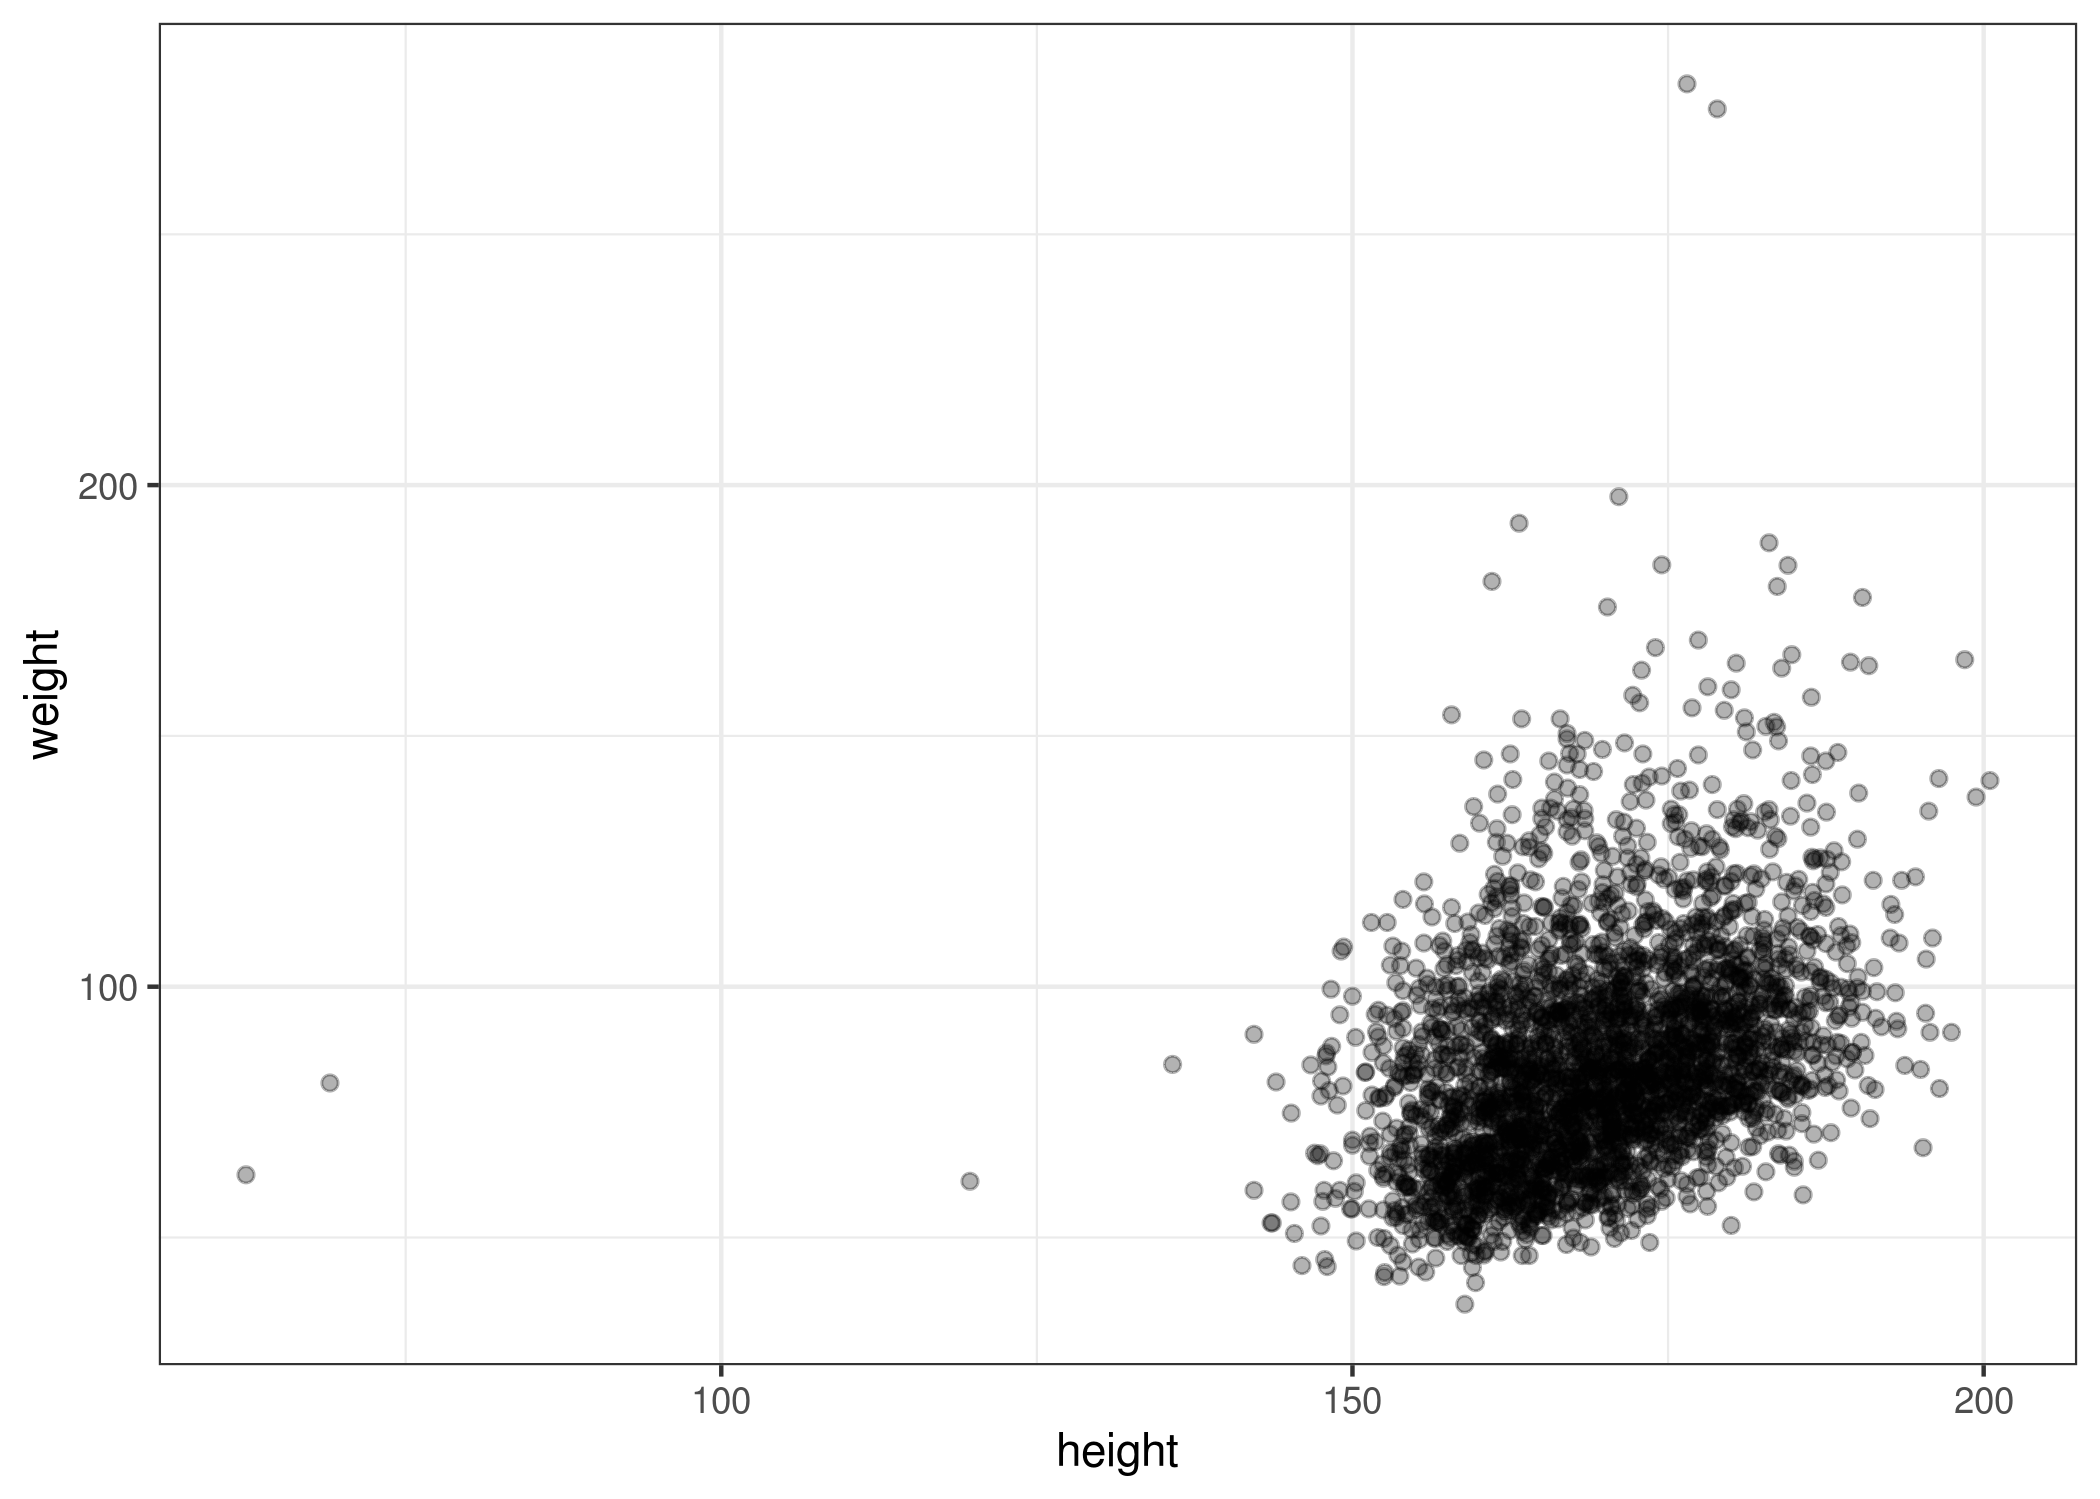
\includegraphics{figures/scatter_height_weight.png}

You can also utilize scatter plots when one of the variables is categorical. For example, we could be interested in the relationship between height and gender.

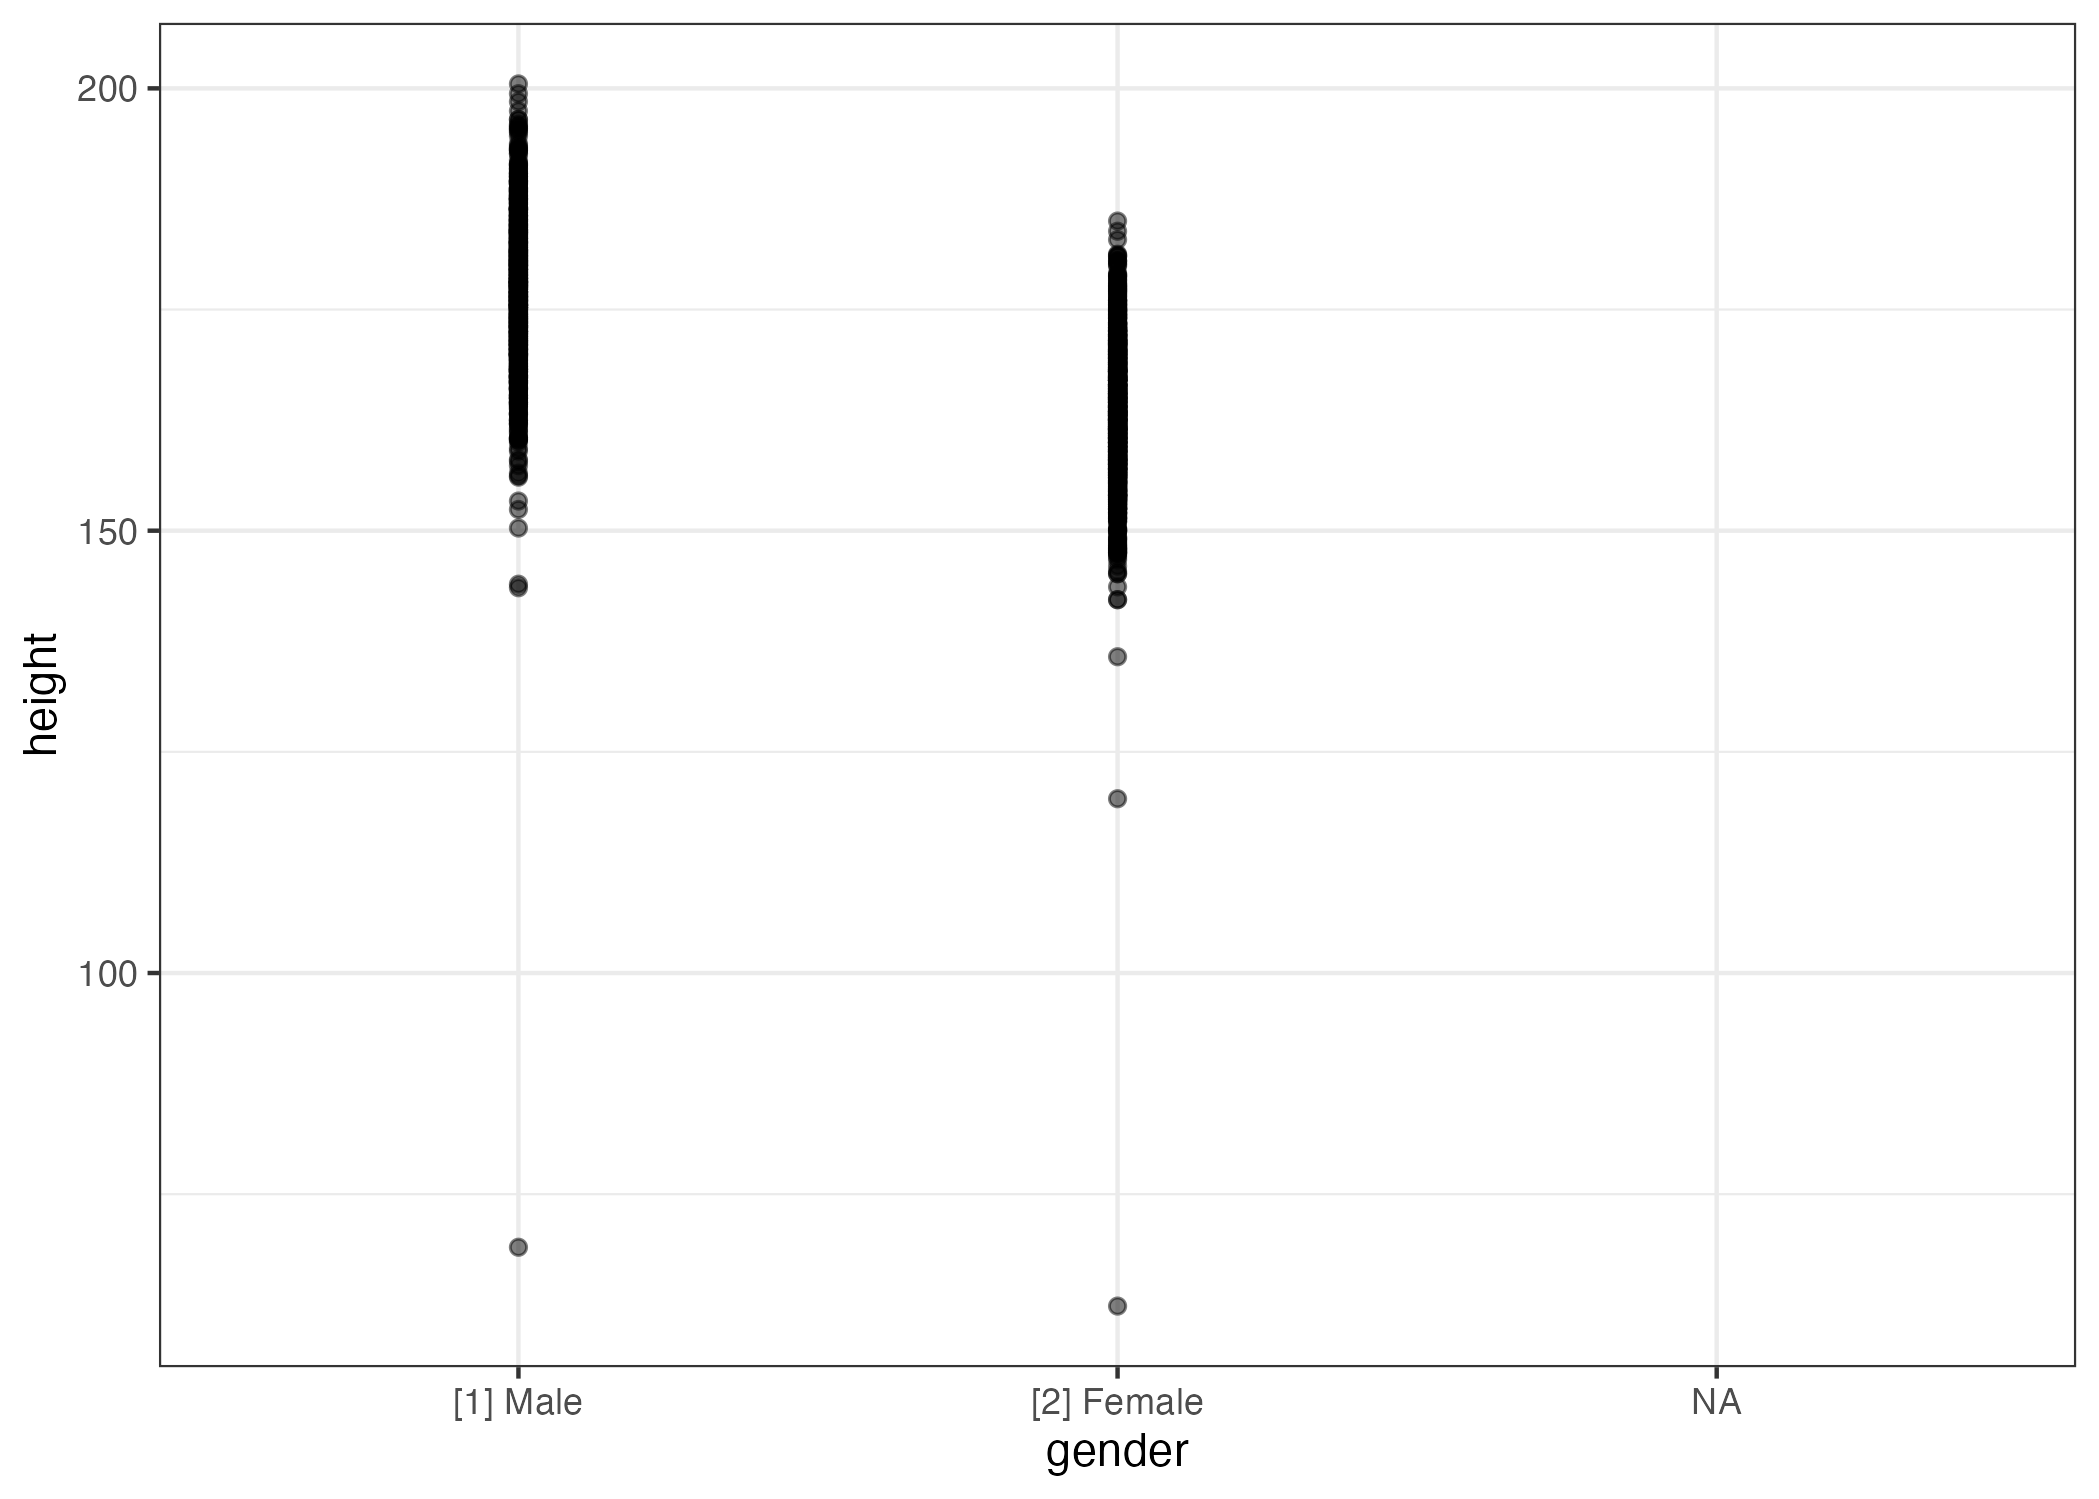
\includegraphics{figures/scatter_gender_height.png}

In this case, it can be beneficial to add a bit of jitter to the plot in the direction of the categorical variable.

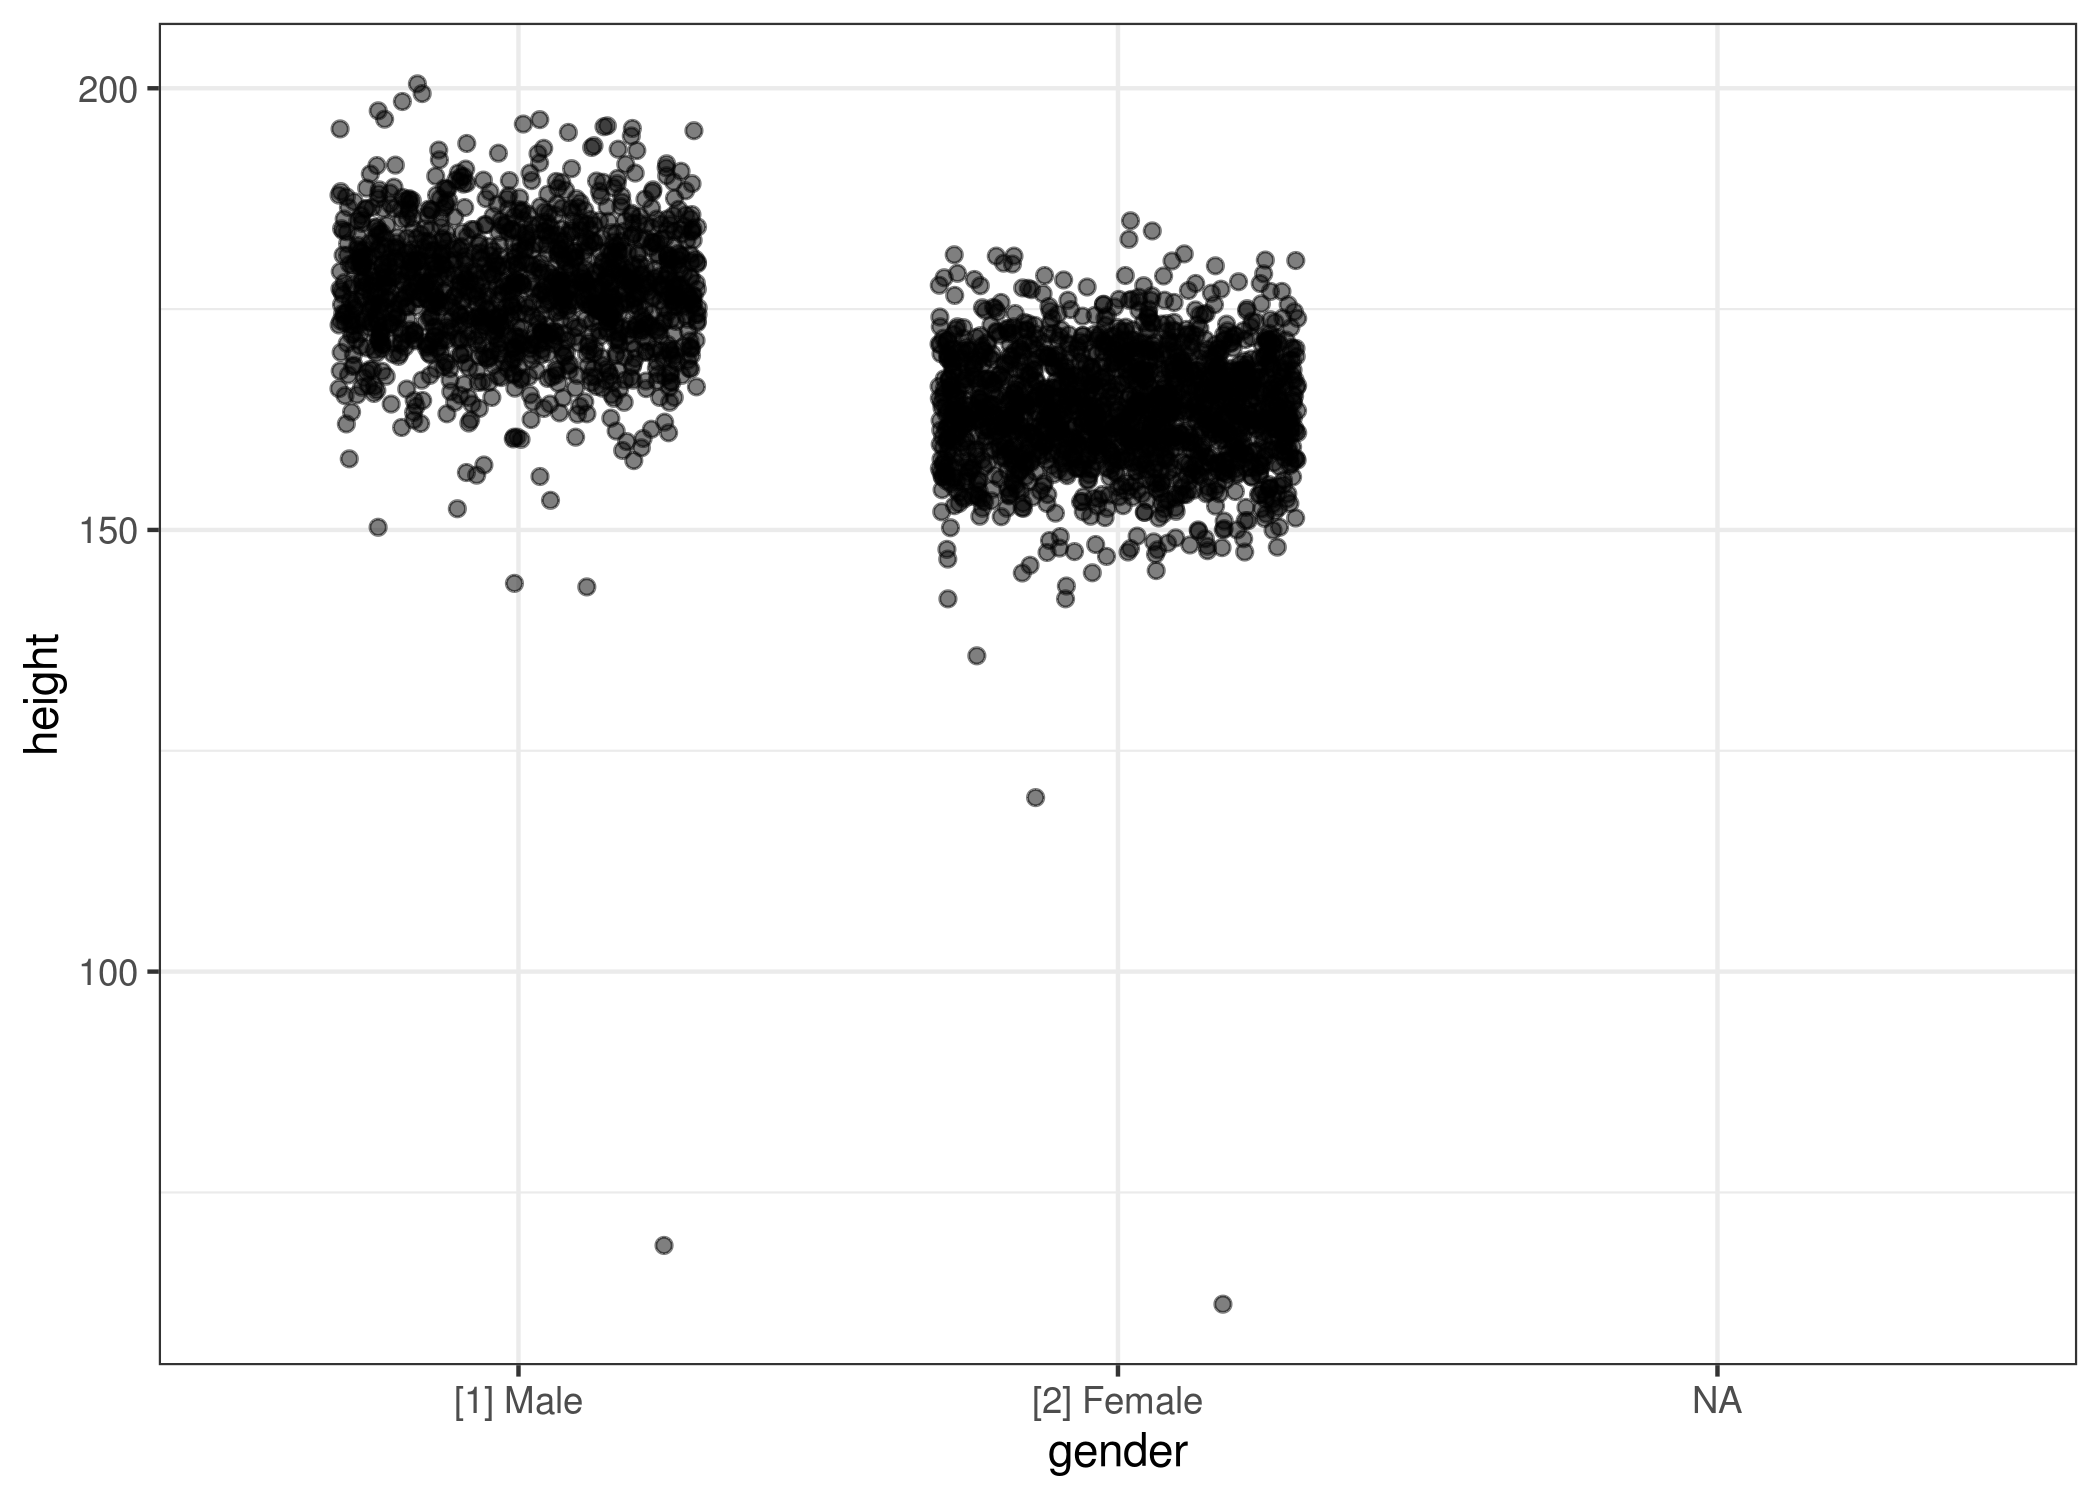
\includegraphics{figures/jitter_gender_height.png}

Even with a bit of jitter, it might be really hard to make anything of a scatter plot in this case, simply because we have ``too much'' data. In such a case, a boxplot might be a better choice.

\hypertarget{boxplots}{%
\subsection{Boxplots}\label{boxplots}}

Boxplots are great when you have a lot of data. They show the data through a set of summaries, namely the quartiles, and indicates if there are any \emph{outliers}. Below are boxplots for the height of the SHOW population by gender.

\includegraphics{figures/boxplot_gender_height.png}

You can use the figure below to decipher the box plot:

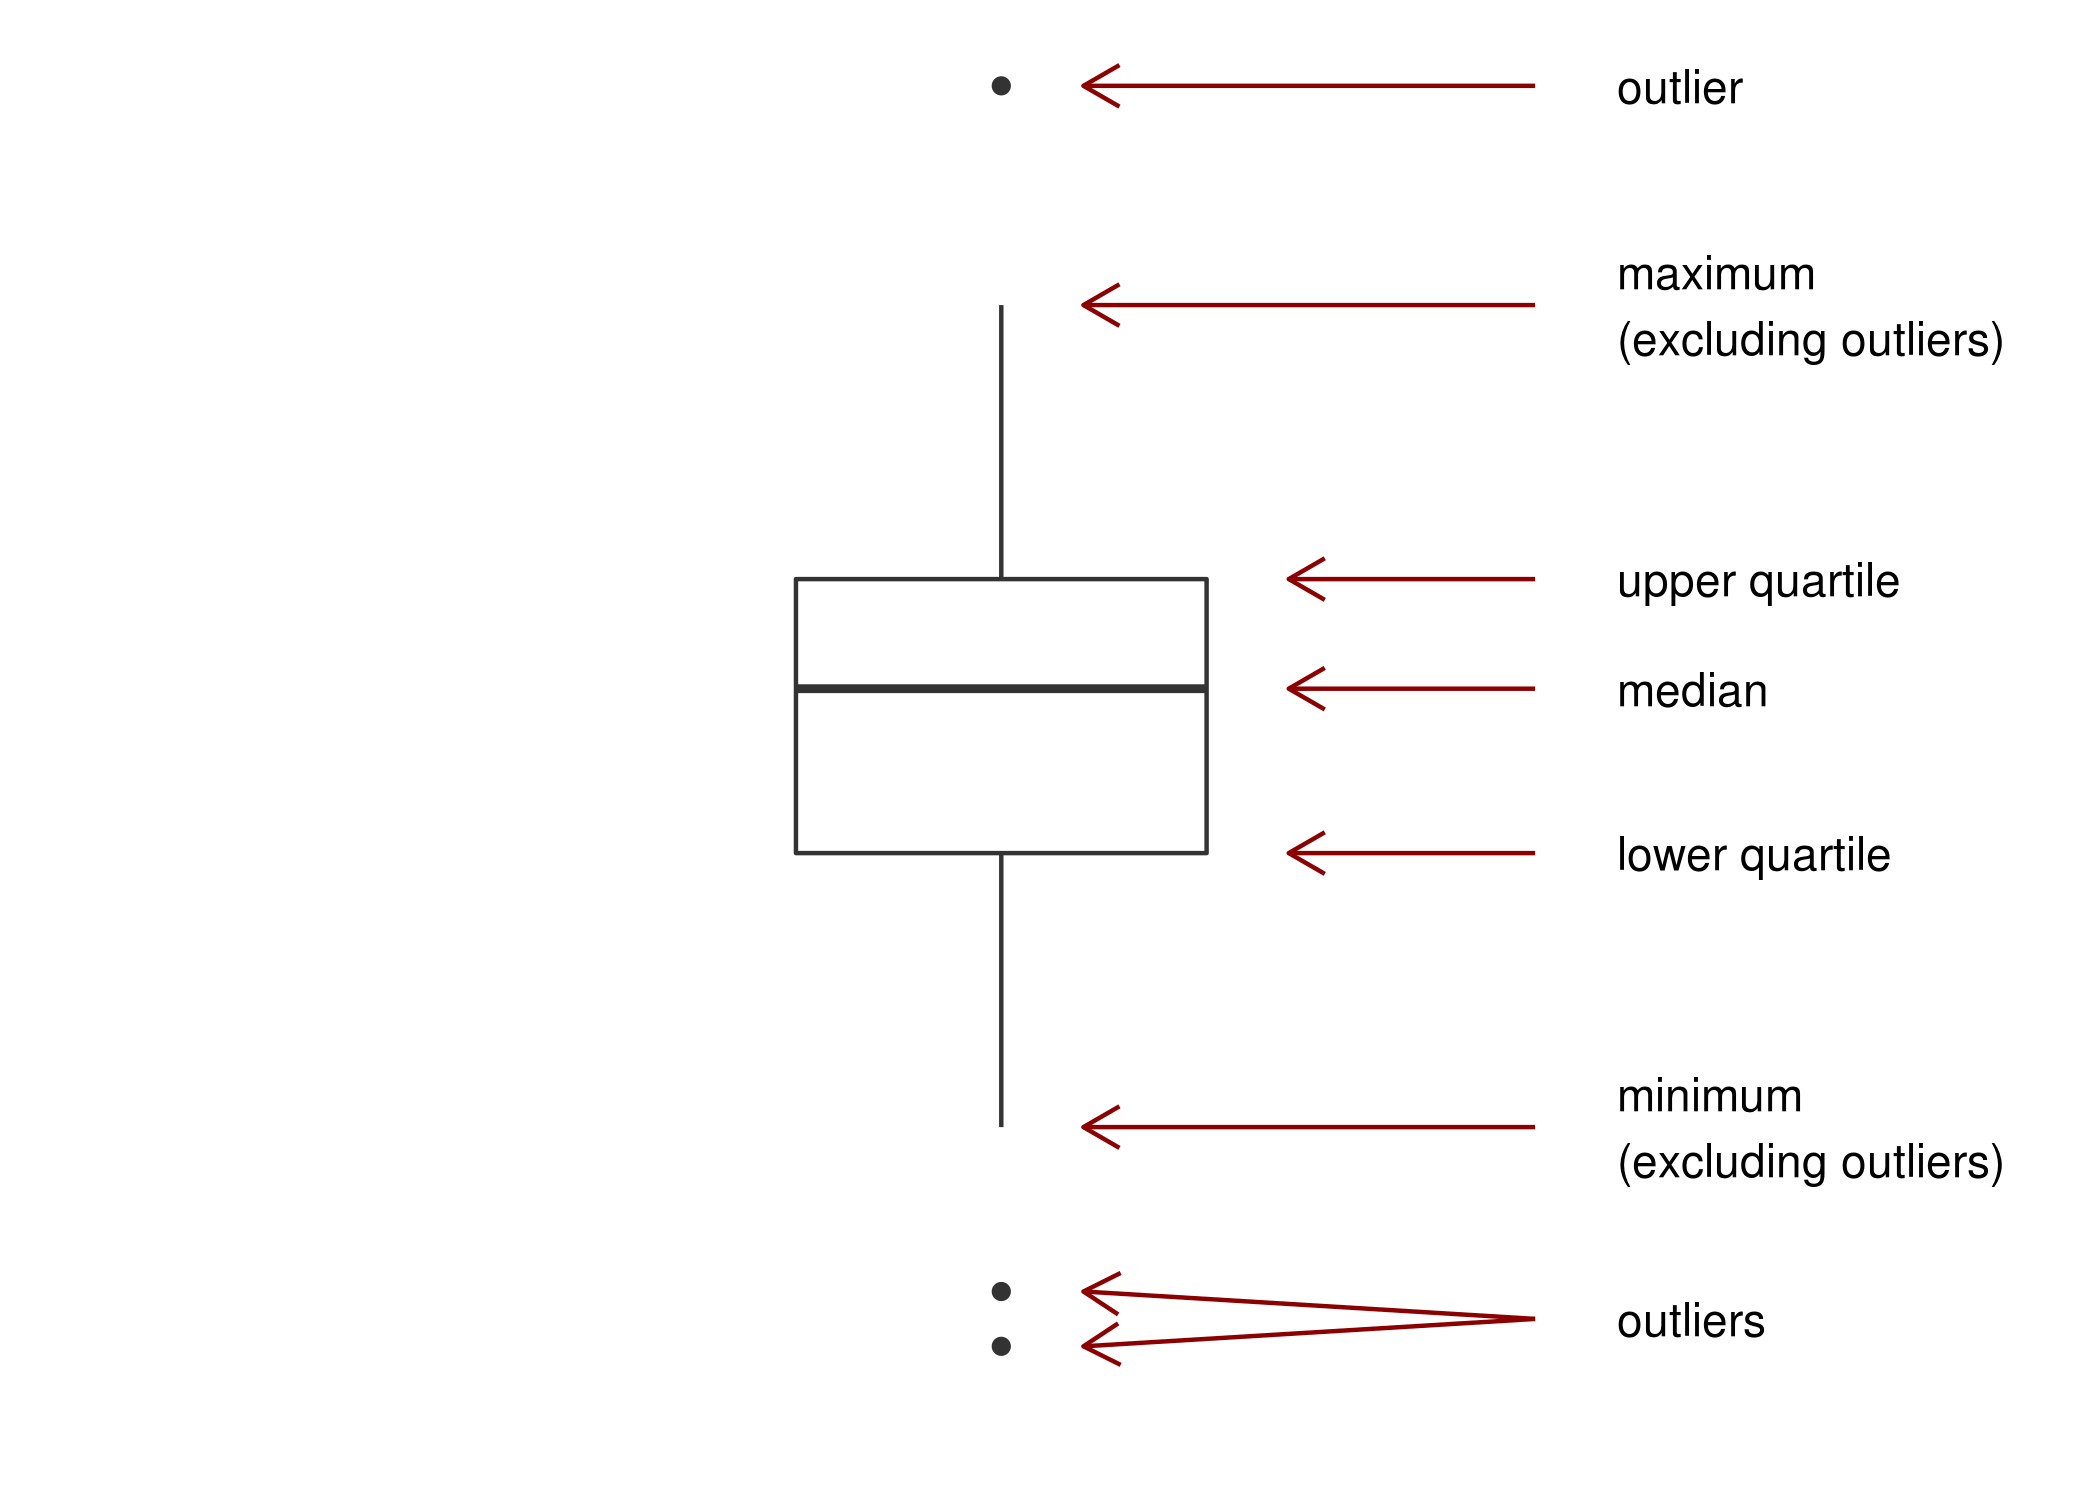
\includegraphics{figures/boxplot_explanation.png}

As you see on the boxplots of the SHOW data, it is a great tool to visualize continuous data when you have a lot of it. In a simple figure we can see that

\begin{itemize}
\tightlist
\item
  the median height is greater for men than women
\item
  there is generally a shift upwards for men compared to women
\item
  the 75\% tallest men are all taller than 75\% of women (compare the bottom of the box for men with the top of the box for women)
\end{itemize}

and much more.

One thing I haven't told you is the answer to a very important, very hard question: ``how do we decide if a data point is an outlier?'' We will simply adopt the practice that a data point is an outlier if it is more than 1.5 times the range of the box from the box. I.e. an observation is an outlier if it is greater than \(Q_3 + 1.5\cdot (Q_3 - Q_1)\) or less than \(Q_1 - 1.5\cdot (Q_3 - Q_1)\).

\hypertarget{histogram}{%
\subsection{Histogram}\label{histogram}}

At first, the \emph{histogram} looks a lot like a bar chart, but there are a few very important differences. Before we go into details, lets take a look at a histogram. Below is a histogram of the depression scores in the SHOW data set.

\includegraphics{figures/bmi_hist.png}

The main differences from a bar chart is that

\begin{enumerate}
\def\labelenumi{\arabic{enumi}.}
\tightlist
\item
  there are no gaps on the x-axis
\item
  the \emph{relative area} of a bar is the proportion of your sample that falls in the interval corresponding to that bar
\end{enumerate}

Later on, we will use the histogram to answer questions like ``what is the probability a randomly chosen individual from the SHOW population has a BMI greater than 40?'' or ``between 20 and 30?'' etc. This is simply done by dividing the area of the bars that are specified (for example all bars with BMI greater than 40) with the total area.

The histogram will be \textbf{super} important to us moving forward, so make sure you know how to decipher it!

\hypertarget{grey-areas}{%
\chapter{Grey areas}\label{grey-areas}}

An example of a variable that could easily be mistaken as categorical is age. Often when we think about age, we think about this in terms of years, or months, or even days. In that sense, age is a variable with a number of possible values that we could technically count -- start with 0, 1, 2, 3, \ldots, 55, 56, 57, \ldots{} . However, this is NOT the natural structure of the variable, but rather a limitation of the way it is measured and recorded. Technically, age is the time from birth till now, which if we could measure it with \emph{infinite} precision, could be any possible number\footnote{positive, real number, for those of you who want to be specific} you can think of.

Many other examples could be provided. In general, what's important to think about is the nature of the variable rather than what is measured. By nature, any measurement is going to be discrete, but some variables are continuous in nature.

\hypertarget{appendix-appendix}{%
\appendix}


\hypertarget{lecture-slides}{%
\chapter{Lecture Slides}\label{lecture-slides}}

\textbf{Lecture 1 (9/12)} \href{./lectures/lecture01/lec01_slides.html}{slides}

\textbf{Lecture 2 (9/26)} \href{./lectures/lecture02/lec02_slides.html}{slides}

\hypertarget{references}{%
\chapter*{References}\label{references}}
\addcontentsline{toc}{chapter}{References}

\bibliography{refs.bib}


\end{document}
